\documentclass[prd,amsmath,amssymb,aps,floats,amsfonts,notitlepage,superscriptaddress,eqsecnum,nofootinbib,10pt]{revtex4-1}
\linespread{1.2}
%\usepackage{booktabs} % for tabular improvments
\usepackage{graphicx}       % Include figure files
\usepackage{dcolumn}        % Align table columns on decimal point
\usepackage{bm}             % bold math
\usepackage{tensor}
\usepackage[utf8]{inputenc}
\usepackage{url}
\usepackage[colorlinks]{hyperref}
\usepackage{color}
\usepackage[usenames,dvipsnames,svgnames,table]{xcolor}
\usepackage{float}
\usepackage{enumerate}
\usepackage[usestackEOL]{stackengine} % package used to write several lines in one box
\allowdisplaybreaks[1]

     % Sarp's extra packages
\usepackage{dcolumn}
	\newcolumntype{.}{D{.}{.}{13}}
	\newcolumntype{d}[1]{D{.}{.}{#1}}
\usepackage{longtable}
\usepackage{subfigure}
\usepackage{rotating}
\usepackage[small,compact]{titlesec}
%%%%%%%%%% New few lines of code are added to fix the TexLive titlesec bug in Ubuntu >= 14.04
\usepackage{etoolbox}
\makeatletter
\patchcmd{\ttlh@hang}{\parindent\z@}{\parindent\z@\leavevmode}{}{}
\patchcmd{\ttlh@hang}{\noindent}{}{}{}
\makeatother
%%%%%%%%%%%%%%%%%%%%%%%%%%%%%%%%%%%%%%%
\usepackage{fancyhdr,amsfonts}
\usepackage{times}
\usepackage{multirow}
\usepackage{sidecap}
\usepackage{eurosym}
\usepackage{setspace}
%\bibliographystyle{apsrev4-1}


\definecolor{CiteColor}{rgb}{0,0.5,0}
\hypersetup{citecolor=CiteColor}
\definecolor{RefColor}{rgb}{0.55,0,0}
\hypersetup{linkcolor=RefColor}
\definecolor{darkgreen}{rgb}{0.2,0.7,0.2}

\newcommand{\beq}{\begin{equation}}
\newcommand{\eeq}{\end{equation}}

\newcommand{\bs}{\mathbf{s}}
\newcommand{\bS}{\mathbf{S}}
\newcommand{\bp}{\mathbf{p}}
\newcommand{\bn}{\mathbf{n}}
\newcommand{\bom}{\boldsymbol{\omega}}
\newcommand{\bOm}{\boldsymbol{\Omega}}
\newcommand{\tilE}{\tilde{E}}
\newcommand{\tilL}{\tilde{L}}
\newcommand{\nn}{\nonumber}
\newcommand{\EE}{E}
\newcommand{\LL}{L}
\newcommand{\KK}{\mathcal{K}}

% Sarp's new commands
\newcommand{\ord}{\mathcal{O}}
\newcommand{\la}{\langle}
\newcommand{\ra}{\rangle}
\renewcommand{\c}{\cos}
\renewcommand{\t}{\theta}
\renewcommand{\b}{\bar}
\newcommand{\f}{\frac}
\newcommand{\pd}{\partial}
\newcommand{\bt}{\beta}
%\newcommand{\s}{\sin}
\newcommand{\ph}{\phi}
\newcommand{\g}{\gamma}
\newcommand{\al}{\alpha}
\newcommand{\La}{\Lambda}
\newcommand{\el}{\ell}
\newcommand{\h}{\hat}
\newcommand{\mrm}{\mathrm}
\newcommand{\Om}{\Omega}
\newcommand{\veps}{\varepsilon}
\newcommand{\be}{\begin{equation}}
\newcommand{\ee}{\end{equation}}
\newcommand{\ba}{\begin{eqnarray}}
\newcommand{\ea}{\end{eqnarray}}
\newcommand{\bi}{\begin{itemize}}
\newcommand{\ei}{\end{itemize}}
\newcommand{\bef}{\begin{frame}}
\newcommand{\ef}{\end{frame}}
\newcommand{\es}{\end{small}}
\newcommand{\Lim}[1]{\raisebox{0.5ex}{\scalebox{0.8}{$\displaystyle \lim_{#1}\;$}}}
\newcommand\T{\rule{0pt}{2.6ex}}       % Top strut for vertical spacing in tables
\newcommand\B{\rule[-1.2ex]{0pt}{0pt}} % Bottom strut

\newcommand{\Delhat}{\hat{\delta}}
\newcommand{\vsp}{\vspace{0.2cm}}

\def\D{\displaystyle}
\def\etal{\textit{et al.}}

\providecommand{\SA}[1]{{\textcolor{DarkBlue}{\texttt{SA: #1}}}}
\providecommand{\SD}[1]{{\textcolor{DarkRed}{\texttt{SD: #1}}}}

\begin{document}

\title{Forecasting Gamma-ray Bursts using Gravitational Waves}

\author{Sarp Akcay}
\affiliation{School of Mathematics \& Statistics, University College Dublin, Belfield, Dublin 4, Ireland.}

\date{\today}

\begin{abstract}
We explore the intriguing possibility of employing future ground-based gravitational-wave interferometers to detect the inspiral of binary neutron stars early enough to alert the electromagnetic observatories so that a gamma-ray burst (GRB) can be observed in its entirety from its very start.
We quantify the ability to predict a GRB by computing the time a binary neutron star (BNS) system takes to inspiral from a its moment of detection to its final merger. We define the moment of detection to be given when the inteferometer network accumulates a signal-to-noise ratio of 15. %for the BNS inspiral.
For our computations, %of advance warning times, 
we specifically consider BNS systems at luminosity distances of (i) $D\le200\,$Mpc in the three-interferometer Advanced-LIGO-Virgo network of 2020, and (ii) $D \le 1000\,$Mpc in the Einstein Telescope's B and C configurations. 
In the case of Advanced LIGO-Virgo we find that we may at best get a few minutes of warning time thus we expect no forecast of GRBs in the 2020s. 
On the other hand, we demonstrate that Einstein Telescope will provide us with warning times as long as a few hours, more specifically, greater than an hour
for BNS inspirals closer than roughly 600\,Mpc. Taking this luminosity distance to be our horizon distance, 
we show that we expect to forecast $\gtrsim \ord(10^2)$ GRBs in the 2030s using the C configuration of Einstein Telescope.
We reapply our computation to binary black hole - neutron star inspirals and find that we expect 1 to 3 tidal disruption events 
to be forecast by the same detector.
%Our main conclusions are: (i) we expect ALV network to forecast 1 to 3 GRBs in the 2020s, (ii)

\end{abstract}
\maketitle


\section{Introduction}\label{Sec:Intro}
The 6.95\footnote{There have thus far been six detections with $5\sigma$ statistical significance and one additional event, LVT151012 \cite{TheLIGOScientific:2016pea}, with $2\sigma \simeq 95\%$ significance hence 6.95 overall.} 
gravitational-wave merger events detected by the Advanced Ligo-Virgo network have firmly established gravitational-wave astronomy
as an observational science \cite{TheLIGOScientific:2016pea, Abbott:2017gyy, Abbott:2017oio, Abbott:2017vtc, GW170817}. 
Though the first event of 14 September 2015 (GW150914 \cite{GW150914}) will always be the ``poster-child'' of this field,
the icing on the cake was the 17 August 2017 (GW170817 \cite{GW170817}) event involving the inspiral and merger of a binary neutron star system with a prompt gamma-ray burst (GRB170817A) detected 1.7 seconds after the coalescence by the Fermi Gamma-ray Burst Monitor \cite{Fermi}{\bf FIX ME} and by the International Gamma-Ray Astrophysics Laboratory (\cite{Savchenko:2017ffs}, {\bf Svinkin, D., et al. 2017, GCN, 21515; Savchenko, V., et al. 2017, GRB
Coordinates Network, 21507}).
The Advanced-LIGO-Virgo network's initial source localization to within $\sim 31\,\text{degree}^2$ in the Southern skies
enabled astronomers to locate the electromagnetic counterpart in the galaxy NGC 4993 less than 11 hours after the merger, 
first picked up by the One-Meter, Two Hemisphere team \cite{Coulter:2017wya} {\bf Coulter, D. A., et al. 2017, GCN, 21529, 21567}.
This subsequently launched the largest-ever campaign of multi-messenger astronomy across the entire electromagnetic (EM) spectrum still ongoing
more than half a year after the initial GRB \cite{GBM:2017lvd}. 

GW170817 was initially identified by the LIGO-Hanford interferometer (H1) 
using a template bank of gravitational waveforms computed within the framework of post-Newtonian theory \cite{Buonanno:2009zt, Blanchet_LRR}.
The inspiral swept across the Advanced Ligo-Virgo (ALV) network's bandwidth from $\sim 30\,$Hz to $\sim 2\,$kHz in 57 seconds
executing $\sim 3000$ GW cycles and accumulating a network signal-to-noise ratio of 32.4 with a false-alarm rate of one per $8.0\times 10^4$ years \cite{GW170817}. 
The total mass of the system was inferred to be $2.74^{+0.04}_{-0.01} M_\odot$ with component masses in the range $1.17-1.60 M_\odot$ consistent
with neutron stars.
Moreover, both the GW and EM observations are consistent with a source luminosity distance of $\sim 40\,$Mpc
and support the hypothesis that GW170817 resulted from the inspiral and merger of two neutron stars, 
which then caused the prompt short-hard gamma-ray burst (GRB170817A) in NGC4993 as first suggested by Ref.~\cite{Eichler:1989ve}. 

One week after GW170817, the ALV network was taken offline for upgrades for the third observation run (O3) 
scheduled to start in Autumn 2018 with roughly twice the sensitivity of O2.
In addition, the Japanese cryogenic interferometer KAGRA (\cite{KAGRA, KAGRA2}) will start its test runs in 2018-2019 and reach design sensitivity circa 2021-2022 \cite{Akutsu:2017thy, Aasi:2013wya}. By 2025, LIGO-India detector will join the global interferometer network hence improving both the overall sensitivity and the sky-localization capabilities \cite{Aasi:2013wya}.
Around this time, the construction of the first third-generation ground-based interferometer, Einstein Telescope, will begin in Europe \cite{ET_doc}. 
The US is currently considering a mid-2020s update called LIGO-Voyager \cite{LIGO_Voy} and a more ambitious 40\,km long interferometer dubbed The Cosmic Explorer \cite{CE}.
All of these near-future improvements to the GW-detector network beg a simple question: can we detect the inspiral of a binary neutron star system
early enough to witness a gamma-ray burst as it happens? In other words, can we forecast GRBs using GW detections?

The short answer is in the affirmative. The long answer is still affirmative, but depends on many factors such as source distance and sky position, detector sensitivity and orientation. One also needs to account for the fact that GRBs are thought to be collimated emissions with narrow outburst angles \cite{Kumar:2014upa}.
As such, most GRBs that occur in the universe are electromagnetically undetectable. Fortunately, this was not the case with GRB170817A, 
but even for a reasonable GRB jet opening angle of $\sim 10^\circ$, we expect to observe $\sim 10\%$ of neutron star mergers as GRBs \cite{Patricelli:2016bkt}. 
However, it is possible that some of the near-Earth pointing short hard GRBs may be observed as long-duration GRBs or X-ray flashes thus increasing this percentage \cite{Bucciantini:2011kx}.

Given the sensitivities of interferometers to date, efforts have thus far mostly focused on reducing the latency of EM follow-ups, 
i.e., the lag time between the merger and the alerting of the EM observatories. 
LIGO-Virgo science runs in 2009-2010 yielded a latency of $\sim 30$ to $60\,$minutes \cite{Abbott:2011ys} (no detections).
In the case of GW170817, the latency was 40\,minutes and $36^{+1.7}\,$seconds \cite{GBM:2017lvd}.
It then took an additional $\sim 10$ hours to locate the optical transient designated AT 2017gfo.

Here, we are interested  in exploring the predictive power of near-future ground-based GW detectors thus leave the task of reducing the latency to the experts.
More specifically, we wish to find out how much early warning the GW detectors can provide us before the merger/GRB.
Ref.~\cite{Cannon:2011vi} approached this from an algorithmic perspective by developing computationally inexpensive methods to detect inspiral
signals in GW data to provide early-warning triggers \emph{before} the merger.
We instead focus on the forecasting capabilities of the ground-based interferometers at their \emph{full design} sensitivity by computing the time lag
between the merger and the detection time defined in terms of a certain threshold SNR.
To this end, we consider the $\sim 2020$ ALV network composed of three L-shaped interferometers operating at their design sensitivities
and Einstein Telescope of 2030s.
Ref.~\cite{Nissanke:2012dj} investigated the capabilities of three to five-interferometer detector networks of 2020s in terms of their horizon distance
to inspiralling BNSs and their sky-localization of these sources. Our work here is somewhat complementary in the sense that we are mostly concerned with
advance warning times.

We compute the advance warning times via the following procedure: 
(${i}$) We start with a GW source presumed to be an inspiralling BNS at a certain luminosity distance. %$D$.
(${ii}$) We determine the frequency at which the source enters a given interferometer's bandwidth. 
In order to more faithfully represent a network such as ALV --- consisting of three separate interferometers which have different
orientations and positions --- we employ root-mean-square averages over sky-position and polarization angles,
and assign the interferometers angle-averaged sensitivities.
%which reduce an individual interferometer's sensitivity to a particular source. 
(${iii}$) We determine the detection time by computing the frequency at which the network's accumulated SNR for the BNS inspiral equals 15.
($iv$) We define the advance warning time to be the remaining inspiral time to the merger from the instant of detection.
We repeat this procedure for BNSs at luminosity distances varying from 50\,Mpc to 1\,Gpc with the smaller values intended for the ALV network and 
the larger ones for Einstein Telescope.
%KAGRA 152Mpc range (K. Somiya, ET meeting at Birmingham, 2017)

Our computation is based on the leading-order Newtonian evolution of the quadrupole moment of a binary system 
composed of two point masses in a quasi-circular orbit.
We supplement this with results from post-Newtonian theory up to 3.5 post-Newtonian order \cite{Blanchet_LRR}.
The strong-field dynamics of BNS evolution is a very complex and complicated problem requiring fully relativistic, magnetohydrodynamic codes 
with neutrino transport running on large-scale computing clusters and taking up to millions of CPU hours 
(see Ref.~\cite{Faber:2012rw} for a review, and Refs.~\cite{Kyutoku:2017voj, Zappa:2017xba} for the latest developments and references therein).
Despite its simplicity, our leading-order treatment is more than sufficient to provide reliable estimations of advance warning times.
We back this claim up with an extensive list of computations showing how much each of our approximations affects the inspiral time.
Let us emphasize that this article is intended as a pedagogical introduction to gravitational-wave astronomy written at a level accessible to
Ph.D. students, advanced undergraduates, and colleagues in astronomy and/or astrophysics who wish to learn more about the basics.
Be that as it may, even the experts might find our results motivating and exciting.

This article is organized as follows. Sec.~\ref{sec:BNS_inspiral} introduces the formulation for the leading-order evolution of the binary inspiral.
Sec.~\ref{sec:IFO_response} details the interferometer response to GWs based on topology.
Sec.~\ref{sec:idealizations} lists the various idealizations we employ to simplify our treatment and supplies justification for each.
Sec.~\ref{sec:GW170817} tests our model network and evolution using the parameters of GW170817 and the corresponding GW data.
Sec.~\ref{sec:results} contains our main results presented as advance warning times in Tables~\ref{table:LIGO2020}, \ref{table:ET} 
as well horizon distances and event rates in Table~\ref{table:horizon}.
In Sec.~\ref{sec:BH_NS}, we reapply the above procedure to black hole - neutron star inspirals to see whether or not 
future detectors can forecast a tidal disruption event, for which we summarize our findings in Table~\ref{table:ET_BH_NS}.

We reserve the symbol $f$ to denote the GW frequency of the dominant quadrupole mode, which is twice the orbital (Keplerian) frequency $f_K$. 
Relatedly, we define the following angular frequencies: $\omega = 2\pi f, \Omega=2\pi f_K$ with $\omega=2\Omega$.
We employ the $\simeq$ symbol for the numerical values of quantities with infinite decimal expansions which we usually truncate at four significant digits,
e.g., $\pi \simeq 3.142$.
The $\approx$ symbol is reserved for approximations, whereas $\sim$ denotes rather rough order-of-magnitude equalities, e.g., $\pi \sim \ord(1)$. %Kepler's third law: $f_K^2\sim r^{-3}$.
Overdots denote time derivative with respect to detector-frame time, e.g., $\dot{E} =dE/dt$. Unless otherwise noted, we use standard SI units.

\section{Binary systems composed of neutron stars}\label{sec:BNS_inspiral}
\subsection{Newtonian evolution of BNS}
For us, the starting point for the evolution of a binary under the emission of GWs is the expression for the power generated given by 
%for the generated by the time-variance of the mass quadrupole moment
%
\be
\dot{E} = \f{G}{5c^5}\langle \dddot{Q}_{ij}\dddot{Q}_{ij} \rangle \label{eq:Edot_quadrupole}\, .
\ee
%
This is the celebrated Einstein quadrupole formula. 
Here, $Q_{ij}$ is a trace-reversed mass quadrupole moment which
is the dominant contribution to the power generated %in gravitational radiation
by a system with changing mass moments. 

Here, we are specifically interested in the motion of two point masses in bound motion around a common center of mass.
Labelling the masses by $m_1 \le m_2$, we have, for a binary in a circular orbit with Keplerian angular frequency $\Omega$ and separation $2r$,
%
\be
\dot{E} = \f{32}{5}\f{G\mu^2}{c^5}\, r^4 \Omega^6\label{eq:Edot}
\ee
%
where $\mu= m_1 m_2/M$ is the reduced mass and $M=m_1+m_2$ is the total mass. 
We justify our simplification of motion to circular orbits in Sec.~\ref{sec:idealizations}.
%Our assumption of the circularity of the motion is well justified in 

An important quantity in GW astronomy is the chirp mass of the binary given by
%
\be
M_c = \mu^{3/5} M^{2/5} = \f{(m_1 m_2)^{3/5}}{(m_1+m_2)^{1/5}} \label{eq:chirp_mass}\, ,
\ee
%
which turns Eq.~(\ref{eq:Edot}) into
%
\be
\dot{E} = \f{32}{5}\f{c^5}{G} \left(\f{G M_c\, \omega}{2c^3}\right)^{10/3}, \label{eq:Edot2}
\ee
%
where, recall $\omega=2\Omega$ is the angular frequency of the quadrupolar GWs. 
The quantity in parantheses in Eq.~(\ref{eq:Edot2}) is ubiquitous in post-Newtonian theory and is
referred to as the dimensionless inverse separation $x$.
As $x\sim v^2/c^2$, it is used to keep track of post-Newtonian orders and we can from in Eq.~(\ref{eq:Edot2}) that $\dot{E}\sim x^5$. 
%hence the common statement in the literature saying that gravitational radiation starts 

The energy generated by the acceleration of the masses is radiated away in GWs,
which makes the total energy of the binary more negative, i.e., the orbit becomes more bound. 
Since the total energy is given by
%
\be
E_b = -\frac{G m_1 m_2}{2r}\, . \label{eq:binding_energy1}
\ee
%
$\dot{E}_b < 0$ implies the orbital radius must decrease in time. 
Using Kepler's third law, $ \Omega^2 = G M r^{-3}$ and Eq.~(\ref{eq:chirp_mass}) we obtain
%
\be
E_b = -\left(\f{G^2 M_c^5 \omega^2}{32}\right)^{1/3}, \label{eq:binding_energy2}
\ee
%
Energy conservation dictates that $\dot{E}=-\dot{E}_b$. Using the chain rule to determine $\dot{E}_b$ from Eq.~(\ref{eq:binding_energy2})
and setting the resulting expression equal to Eq.~(\ref{eq:Edot2}) yields $\dot{\omega}$ as a function of $\omega$ and various constants.
Translating this expression using $\omega=2\pi f$ we arrive at the standard expression for the GW frequency evolution
%%
%
\be
\dot{f} = \f{96}{5}\pi^{8/3} \f{(G M_c)}{c^5}^{5/3}\, f^{11/3} \label{eq:fdot}
\ee
%
This can be integrated straightforwardly after defining a new time variable $\tau\equiv t_\text{coal}-t$ that equals zero when the neutron stars coalesce.
We can now define an inspiral time at a given GW frequency
%
\be
\tau_\text{insp}(f) = \f{5}{256\pi}\f{c^5}{(\pi G M_c)^{5/3}} \,f^{-8/3}\label{eq:tau_insp}\, ,
\ee
%
%
%\be
%\tau_\text{insp}(f) \equiv \f{5}{256\pi}\f{c^5}{(\pi G M_c)^{5/3}}\left[ f^{-8/3}-f_\text{ISCO}^{-8/3}\right]\label{eq:tau_insp} \, .
%\ee
%
which we can rewrite as follows
%
\be
\tau_\text{insp}(f) \simeq 2.18\,\text{s} \, \left(\f{1.21 M_\odot}{M_c}\right)^{5/3}\,\left(\f{100\,\text{Hz}}{f}\right)^{8/3}, \label{eq:tau_insp2}
\ee
%
where $1.21 M_\odot$ is the chirp mass corresponding to $m_1=m_2=1.4 M_\odot$.

We can also compute the number of GW cycles over the course of an inspiral. Given that the orbital period $T(t)$ varies over a much larger time scale than T itself
we can write
%
\be
\mathcal{N}_\text{cyc}(f) = \int_f^{f_\text{max}} \f{f}{\dot{f}}\, df =\f{1}{32\pi} \f{c^5}{(\pi G M_c)^{5/3}}\left[ f^{-5/3}-f_\text{max}^{-5/3}\right] \label{eq:Ncyc1}
\ee
%
We now introduce a cut-off for the inspiral imposed by the frequency of the innermost stable circular (ISCO) orbit in Schwarzschild spacetime
\be
\Omega_\text{ISCO} = \f{c^3}{6^{3/2} G M} \label{eq:Sch_f_isco}.
\ee
%
%
We will see in Sec.~\ref{sec:idealizations} that $f_\text{ISCO} \sim \mathcal{O}(1000)\,$Hz for a system with $M\approx 2 M_\odot$. Moreover, the frequencies of interest for our advance warning time estimations will be $\lesssim \mathcal{O}(10)\,$Hz
meaning that $f^{-5/3} \gg f_\text{ISCO}^{-5/3}$. Therefore, at the leading (Newtonian) order, the number of GW cycles can be approximated by
%
\be
\mathcal{N}_\text{cyc}(f) \simeq \f{1}{32\pi} \f{c^5}{(\pi G M_c)^{5/3}}\, f^{-5/3} \, . \label{eq:Ncyc2}
\ee
%
Restoring some familiar numbers in this expression yields
%
\be
\mathcal{N}_\text{cyc}(f)\simeq 1.6\times 10^4 \left(\f{10\,\text{Hz}}{f} \right)^{5/3}\,\left(\f{1.21 M_\odot}{M_c}\right)^{5/3}\label{eq:Ncyc3}\, .
\ee
%
This expression is quite telling: if a ground-based interferometer picks up an
inspiralling BNS at $f=10\,$Hz then there will be $\gtrsim \ord(10^4)$ GW cycles in the detector's data stream until the merger.

Another useful relation is how the inspiral time scales with respect to the orbital radius corresponding to the observed GW frequency.
From Kepler's third law, we immediately have $\dot{r}/r= -2\dot{\Omega}/(3\Omega)=-2\dot{f}/(3f)$, which, via Eq.~(\ref{eq:tau_insp}),
yields $\dot{r}/r= -1/(4\tau)$ which integrates to
%
\be
r(\tau)=r_i \left(\f{\tau}{\tau_i}\right)^{1/4}\label{eq:r_of_tau},
\ee
%
where $r_i, \tau_i=t_\text{coal}-t_i$ are the initial radius and time that the BNS
is ``picked up'' by a detector. Solving $\tau(f_i)=\tau_i$ for $f_i=\Omega_i/\pi$ using Eq.~(\ref{eq:tau_insp}) and rewriting $\Omega_i$ as a function of $r_i$ via
Kepler's third law gives us
%
\be
\tau_i = \f{5}{256}\, \f{c^5 r_i^4}{G^3 M^2 \mu}\simeq 9.829\times 10^6\,\text{yrs}\, \left(\f{T}{1\,\text{hr}}\right)^{8/3} \left(\f{M_\odot}{M}\right)^{2/3}\,\left(\f{M_\odot}{\mu}\right) \label{eq:tau_of_r}.
\ee
%

Let us now turn our attention to the GWs generated by the inspiral.
The GWs themselves actually are tensor distortions $h_{\mu\nu}$ of the flat Minkowski
spacetime propagating at the speed of light.
In more technical terms, they satisfy $\Box h_{\mu\nu} = 0$, i.e., the flat spacetime sourceless wave equation
meaning that we are considering the solutions far from the GW source, in the so-called wave zone defined by the condition $ c/f \ll D$.
In a suitable gauge, such as the commonly used TT (transverse-traceless) gauge, it can be shown that
there exist only two physical degrees of freedom which manifest themselves
as two independent polarization amplitudes $h_+$ and $h_\times$. %when interacting with masses away from the source.
For a circular binary at a distance $D$ these states read
%
\begin{align}
 h_+(t) &= h_c(t)\, \left(\f{1+\cos^2\iota}{2}\right)\, \cos[\Phi_\text{N}(t)],\label{eq:hplus_TD}\\
 h_\times(t) & =h_c(t)\,\cos\iota \sin[\Phi_\text{N}(t)]\label{eq:hcross_TD},
\end{align}
%
%
where
%
\be
h_c(t) =\f{4}{D}\left(\f{G M_c}{c^2}\right)^{5/3}\, \left(\f{\pi f(t)}{c}\right)^{2/3} \label{eq:h_c}
\ee
is the characteristic strain.
$\iota=\cos^{-1}(\mathbf{\hat{n}}\cdot{\mathbf{\hat{L}}}) $ is the inclination angle between the line of sight unit vector $\mathbf{\hat{n}} $ and the orbital angular momentum unit vector $\mathbf{\hat{L}}$. 
E.g., for an orbit seen edge on, $\iota = \pi/2$ which is actually the case of a purely plus-polarized wave, $h_\times=\cos(\pi/2)=0$.
When $\iota=0$ the orbit is seen face-on and we have a circularly-polarized wave: $\langle h_+ \rangle = \langle h_\times\rangle$ where $\langle \ldots \rangle$
denote time-averages over one orbit. Note that as $f$ increases in time, so does $h(t)$ hence the characteristic ``chirping'' of GW signals.

$\Phi_\text{N}(t)$ in Eqs.~(\ref{eq:hplus_TD}, \ref{eq:hcross_TD}) is the phase of the GWs given by
%
\begin{align}
\Phi_\text{N}(t) &=\int_{t_i}^t dt' \omega(t') \nn\\
&= -2\left(\f{5 G M_c}{c^3}\right)^{-5/8} (t_\text{coal}-t)^{5/8}+ \Phi_0 \, .\label{eq:Phase}
\end{align}
%
$\Phi_0 \equiv \Phi(t=t_\text{coal})$ is an integration constant. The subscript N denotes the Newtonian (leading-order) contribution. 
Higher-order contributions can be added in terms a post-Newtonian series which make up $\lesssim 2\%$ of the total phase.
Although we will include contributions up to and including 2PN to obtain the results of Sec.~\ref{sec:results}, we will not explicitly show these expressions 
which can be found in Ref.~\cite{Blanchet_LRR}.

The nomenclature ``plus'' ($+$) and ``cross'' ($\times$) follows from the effects that passing GWs have on the plane transverse to their direction of propagation.
If we were to conceive of an imaginary detector made up of a circular configuration of point-particles lying in the $x$-$y$ plane, a GW propagating along the $z$ direction would stretch/compress the circular arrangement in a $+$ and $\times$ pattern which is the manifestation of the tidal strain of the GWs on the tranverse plane.
%which is why $h_{+},h_{\times}$ are often called GW strains. 
Next, let us briefly explore how a real detector, i.e., an interferometer, responds to passing GWs.


\section{Interferometer response to gravitational waves}\label{sec:IFO_response}
\subsection{LIGO-Virgo configuration: L-shaped topology}\label{sec:LIGO_topo}
We start by first considering the L-shaped interferometer topology dating back to Michelson.
Although the GWs are described by propagating tensor modes, an interferometer (IFO) can only measure a scalar quantity
known as the response function (or GW strain)
which is a linear combination of the polarizations given by
%
\be
h(t) = F_+(\theta,\phi,\psi) \,h_+(t)+F_\times(\theta,\phi,\psi)\, h_\times(t) , \label{eq:detector_strain}
\ee
%
where
%%
%
\begin{align}
 F_+ &=\f{1}{2}\left(1+\cos^2\theta\right)\cos2\phi\cos 2\psi-\cos\theta \sin2\phi \sin2\psi \label{eq:F_plus},\\
 F_\times &=\f{1}{2}\left(1+\cos^2\theta\right)\cos2\phi\sin2\psi+\cos\theta \sin2\phi \cos2\psi \label{eq:F_cross}
\end{align}
%
%%
%$F_+, F_\times$ 
are the antenna pattern functions of the detectors; $\theta,\phi$ are the sky coordinates; and $\psi$ is
an additional angle coming from the respective rotations of detectors' frames to source frame. %(there is no need for $\psi$ in the case of a single detector).
%In principle, $\psi$ can be aligned with the polarization of the incoming GWs 
%
We can't apriori know $\theta, \phi,\psi$. However, we can extract their values with some limited precision over the course of an inspiral (preferably of BNS) 
emitting GWs which sweep across the detection band of more than one interferometer over thousands of cycles. This was indeed the case of GW170817
with a source sky localization of 28\,deg$^2$ using data from three inteferometers \cite{GW170817}. 
For our estimations, we will use suitable averages of these angles.
For details on how to obtain Eqs.~(\ref{eq:F_plus}, \ref{eq:F_cross}) see, e.g., Sec.~4.2.1 of Ref.~\cite{SchutzLRR}.

To compute the advance warning times we will need to know how ``loud'' the binaries become as they sweep across the interferometers' band.
This is achieved by computing the signal-to-noise ratio (SNR) of the GWs in the detectors' data stream.
This is done in the frequency domain so we need the Fourier transforms of the time-domain strains of Eqs.~(\ref{eq:hplus_TD}) and (\ref{eq:hcross_TD})
%
\begin{align}
 \tilde{h}_+(f) &= A \, \f{c}{D}\, \left(\f{G M_c}{c^3}\right)^{5/6}\, e^{i \Psi_+(f)}\, \f{1}{f^{7/6}}\,  \f{1+\cos^2\iota}{2}  ,\label{eq:hplus_FD}\\
 \tilde{h}_\times(f) & = A \, \f{c}{D}\, \left(\f{G M_c}{c^3}\right)^{5/6}\, e^{i \Psi_\times(f)}\, \f{1}{f^{7/6}}\, \cos\iota \label{eq:hcross_FD},
\end{align}
%
%
where $A= \pi^{-2/3} \sqrt{5/24}$.
Explicit expressions for $\Psi_{+,\times}$ show that they are out of phase by $\pi/2$
(the details of the Fourier transformation can be found in Sec.~4.5 of Ref.~\cite{Maggiore}).
Accordingly, the Fourier transform of the detector strain (\ref{eq:detector_strain}) is given by
%%
%
\be
\tilde{h}(f) = A\, \f{c}{D}\left(\f{G M_c}{c^3}\right)^{5/6} f^{-7/6}\, e^{i\Psi_\text{N}}\, Q(\theta,\phi,\psi,\iota), \label{eq:strain_FD}
\ee
%
%%
where 
%
\be
Q(\theta,\phi,\psi,\iota) = F_+(\theta,\phi,\psi)\f{1+\cos^2\iota}{2}  + i F_\times(\theta,\phi,\psi) \cos\iota \label{eq:Q},
\ee
%
is the quality factor.
The $i$ in front of $F_\times$ in $Q(\theta,\phi,\psi,\iota)$ is due to the $\pi/2$ phase difference between $+$ and $\times$ modes.
$\Psi_\text{N}$ is the leading-order contribution to the frequency-domain phase
%
\be
\Psi_\text{N}=\Psi_+(f)|_\text{N} = 2\pi f (t_\text{coal}+D/c)-\Phi_0-\f{\pi}{4}+ \f{3}{128}\left(\pi f\,\f{G M_c}{c^3}\right)^{-5/3} \label{eq:phase_FD}.
\ee
%
%
Higher-order contributions up to and including 3.5PN can be found in Ref.~\cite{SchutzLRR}.

The detection criterion we will employ here is quantified in terms of the optimal signal-to-noise ratio (SNR) defined by
%%
%
\be
\rho=\left[ \int_0^\infty d\ln f\, \f{|2\tilde{h}(f)\sqrt{f}|^2}{S_n(f)}\right]^{1/2} \label{eq:SNR},
\ee
%
%%
where $\sqrt{S_n(f)}$ is the {\it amplitude spectral density} (ASD) [also called spectral strain sensitivity] of the detector.
It is usually this quantity that is shown in a typical interferometer strain sensitivity plot with the characteristic strain, $\tilde{h}_c(f)\equiv2\tilde{h}(f)\sqrt{f}$, 
due to various GW sources overlaid for comparison. 
%
%against the amplitudes of various GW sources whose
%ASDs are given by $2\tilde{h}(f)\sqrt{f}$. This particular combination is called the characteristic strain. 
We will show such plots in Sec.~\ref{sec:results}.

Substituting Eq.~(\ref{eq:strain_FD}) into Eq.~(\ref{eq:SNR}) yields
%%
%
\be
\rho^2 = \f{5}{6}\, \pi^{-4/3} \f{c^2}{D^2}\left(\f{G M_c}{c^3}\right)^{5/3}|Q(\theta,\phi,\psi,\iota)|^2 \int_0^{f_\text{ISCO}} d f\, \f{f^{-7/3}}{S_n(f)}\, \label{eq:SNR_v2},
\ee
%
%%
where we truncate the integral at the cut-off frequency of the inspiral $f_\text{ISCO}=\Omega_\text{ISCO}/\pi$.

It remains to compute $|Q(\theta,\phi,\psi,\iota)|^2$. 
Since we can not know the direction of the source a priori, it is appropriate to average over the angles $\theta,\phi,\psi,\iota$ which we compute
%For our computations, we will only work with one detector so we can set $\psi=0$ without loss of generality, which results in
%%
%
%\be
%F_+(\theta,\phi) = \f{1}{2}(1+\cos^2\theta)\cos2\phi, \qquad F_\times(\theta,\phi) = \cos\theta \sin2\phi.
%\ee
%
%%
via the following RMS-averaging integral
%%
%
\be
\langle F^2_{+}\rangle \equiv \f{1}{2\pi}\int_0^{2\pi}d\psi \,\f{1}{4\pi}\int_0^{2\pi} d\phi\,\int_0^\pi d\theta \sin\theta\ F^2_{+}(\theta,\phi,\psi)=\f{1}{5}\label{eq:ang_av}
\ee
%
%%
and likewise $\langle F^2_{\times}\rangle=1/5 $.
Finally, we average over the orbital inclination angle
%
\be
%\langle g(\iota) \rangle = 
\f{1}{2} \int_0^\pi d\iota\sin\iota\left[\left(\f{1+\cos^2\iota}{2}\right)^2+\cos^2\iota\right] = \f{4}{5} .\label{eq:inc_ang_av}
\ee
Thus we have that
%
\be
\langle |Q(\theta,\phi,\psi,\iota)|^2 \rangle_{\theta,\phi,\psi,\iota} = \f{4}{25}\label{eq:RMS_th_ph_ps_iota}.
\ee
%
As angles have zero averages in general, we can think of the RMS as the standard deviation ($\sigma =2/5$). 
Therefore, $2\sigma= 4/5$ above the average (zero in this case) should statistically cover 95\% of the four-dimensional angle space. 
%Finally, we add the case of an optimally-oriented, purely $+$-polarized source ($\psi=0,\iota=0$) that is directly overhead ($\theta=0$) simply resulting in 
%
%\be
%\langle |Q(\theta=0,\phi=0,\psi=0,\iota=0)|^2 \rangle = 1.
%\ee
%
%
%
%\be
%\tilde{H}(f)\equiv  A\,\left\langle\, |Q(\theta,\phi,\psi,\iota)|^2\,\right\rangle^{1/2}\, \f{c}{D}\left(\f{G M_c}{c^3}\right)^{5/6} f^{-7/6}\, . \label{eq:ang_av_strain_FD}
%\ee
%
%%

In a network of $N$ interferometers, the total SNR is defined as follows
%%
%
\be
\rho_\text{tot} = \left[{\sum_{i=1}^N \rho^2_i}\right]^{1/2} \label{eq:SNR_total}
\ee
%
%%
where Eq.~(\ref{eq:SNR_v2}) is employed to compute $\rho_i$ coming from individual interferometers each with a specific quality factor $Q_i$.
Here, instead of working with specific quality factors of the LIGO and the Virgo interferometers, we consider
an \emph{model network} of three detectors ($N=3$), where one interferometer is near-optimally oriented/positioned thus it is at $2\sigma$ above the average.
The second IFO operates at the RMS average; thus its sensitivity is suppressed by a factor $2/5$ compared with $\langle|Q|^2\rangle =1$ case.
It remains to assign a quality factor for the third IFO. We wish to make this operate below the RMS average, % in terms of its orientation and the sky location of the sources,
but it would be pointless to simply set its $\langle|Q|^2\rangle$ equal to zero. We therefore somewhat arbitrarily set $\psi=0,\iota=0$
and introduce the following $\theta,\phi$-only averages
%
\be
 \langle F_+^2\rangle_{\theta,\phi} = \frac{7}{30},\qquad \langle F_\times^2\rangle_{\theta,\phi} = \frac{1}{6}\, 
\ee
yielding
%
\be
\langle |Q(\theta,\phi,\psi=0,\iota=0)|^2 \rangle_{\theta,\phi} = \f{2}{5} \label{eq:RMS_th_phi}.
\ee
Using this value, we assign our below-average third IFO $\langle|Q|^2\rangle^{1/2}=4/5-\sqrt{2/5}\simeq 0.1675$.
%which is essentially a $\{\theta$-$\phi\}$-RMS awayfrom the overall RMS averaged value of 2/5.
This may seem somewhat ad hoc, but it is our way of modeling the Advanced-LIGO-Virgo network of 2020s in which 
the three IFOs will accumulate varying SNRs due to their differing quality factors.
%

Therefore, to represent our multi-interferometer network, we introduce % the norm of the frequency-domain strain (\ref{eq:strain_FD}) 
%%
%
\be
\tilde{H}_i(f)\equiv \tilde{A}_i\, h_0\, f^{-7/6} \label{eq:Hi_s}
\ee
%
%%
for each interferometer, where
%%
%
\begin{align}
%\tilde{A}_i &\equiv A \langle |Q|^2\rangle^{1/2}_i=\f{1}{2}\sqrt{\f{5}{6}}\, \pi^{-2/3} \left\langle\, |Q_i(\theta,\phi,\psi,\iota)|^2\,\right\rangle^{1/2}\quad\text{and} \label{eq:A_tilde}\\
h_0 &= \f{c}{D}\left(\f{G M_c}{c^3}\right)^{5/6} \label{eq:h0}\, .
\end{align}
%
and the $\tilde{A}_i =A\langle|Q|^2\rangle^{1/2}_i $ are given in Table~\ref{table:network_params}. %for $i=1,2,3$. %Clearly, the strain and thus the SNR at each of our imaginary interferometers scales as $\langle |Q|^2\rangle^{1/2}_i$, thus
%%
The SNR for each interferometer can now be written as
%%
%
\begin{align}
\rho_i &= 2\tilde{A}_i\, h_0 \left[\int_0^{f_\text{ISCO}} df\, \f{f^{-7/3}}{S_\text{n}(f)} \right]^{1/2}\label{eq:SNR_i}.
\end{align}
%
We arbitrarily make the following assignments for our network: $h=1, m=2, l=3$ representing high, medium, low strains/SNRs, respectively. 
We summarize our network in the following Table~\ref{table:network_params}.
%%

\begin{table}[h]
\centering
\begin{tabular}{c|c|c|c}
 IFO$_i$ & configuration %& $\langle |Q_i|^2\rangle$ 
 & $\tilde{A}_i$ & $\tilde{H}_i(f)$\\
 %\hline
 \hline
 1 & high ($h$) &  A & $A h_0\, f^{-7/6}$ \T\\
 2 & medium ($m$) & $\tfrac{2}{5}A$ & $ \tfrac{2}{5}A h_0 \, f^{-7/6}$\B\T \\
 3 & low ($l$)  & $\left(\tfrac{4}{5}-\sqrt{\tfrac{2}{5}}\right)A$ & $ \left(\tfrac{4}{5}-\sqrt{\tfrac{2}{5}}\right)A h_0 \, f^{-7/6}$\B \\
 \hline
\end{tabular}
\caption{%The averaged quality factors $\langle|Q|^2\rangle$ of 
Our model for the Advanced-LIGO-Virgo network ca. 2020. %of three L-shaped interferometers (IFOs). 
Column four lists the magnitude of the strain for each IFO via Eq.~(\ref{eq:Hi_s}).
``Configuration'' describes how ideally oriented/positioned an IFO is with respect to a compact binary source. 
High is $2\sigma$ above the average as explained above.
Medium is the RMS-averaged (one $\sigma$) response. Recall $A= \pi^{-2/3} \sqrt{5/24}$. 
%Note that for an interferometer where the angle between the arms is $\alpha$, $A$ rescales to $A\sin\alpha$.
}\label{table:network_params}
\end{table}
%
%
We can now write the total SNR for our network
%%
%
\begin{align}
\rho_\text{tot} &= \sqrt{\rho^2_h+\rho^2_m+\rho^2_l} \label{eq:SNR_total_3IFOs} .
%	      &= 2A h_0 \sqrt{1+\tfrac{2}{5}+\tfrac{4}{25}} \left[\int_0^{f_\text{ISCO}} df\, \f{f^{-7/3}}{S_\text{noise}(f)}\right]^{1/2}\nn\\
%	      &= \sqrt{\frac{13}{10}}\,\pi^{-2/3}\,\f{c}{D}\left(\f{G M_c}{c^3}\right)^{5/6}\left[\int_0^{f_\text{ISCO}} df\, \f{f^{-7/3}}{S_\text{noise}(f)}\right]^{1/2} \label{eq:SNR_total_3IFOs_v2}.
\end{align}
%
%%
%Although we made several simplifying assumptions to obtain $\rho_\text{tot}$, these should not affect our total SNR estimation too much.
%For example, averaging over all the angles underestimates the SNR of an interferometer with a near-ideal orientation with respect to the incoming GWs
%while also overestimating the SNR of a badly oriented detector. Rewriting Eq.~(\ref{eq:SNR_total}) as Eq.~(\ref{eq:SNR_total_3IFOs}) compensates
%for these.
We will start Sec.~\ref{sec:results} by testing our network with GW170817 whose signal got picked up by the LIGO detectors around $f=30$\,Hz.
So we will change the lower limit of the integral in Eq.~(\ref{eq:SNR_total_3IFOs}) from $0$ to $30$.
For our advance warning times we will further use separate initial frequencies for each inteferometer as we will explain in Sec.~\ref{sec:results}.


\subsection{Einstein Telescope configuration: triangular topology}\label{sec:ET_topo}
Current design of Einstein Telescope is based on a [equilateral] triangular configuration with 10\,km armlengths \cite{ET_doc}.
Within this equilateral triangle, ET will consist of three V-shaped cryogenic interferometers housed underground to
sigificantly reduce seismic and gravity-gradient noises \cite{ET_doc}.
This closed topology will allow the detector to form a null stream completely devoid of a signal \cite{Sathyaprakash:2012jk},
which can be used to rule out spurious events \cite{Wen:2005ui}.
As we will show below, the response function and the quality factor of the triangular configuration are independent of the azimuthal angle $\phi$
hence ET will have no blind spots \cite{Regimbau:2012ir}.
However, the $60^\circ$ arm separation reduces the strain of a V-shaped interferometer by a factor of $\sin 60^\circ=\sqrt{3}/2$ compared
to an L-shaped interferometer. So for a single V-IFO the antenna patterns of (\ref{eq:F_plus}, \ref{eq:F_cross}) become
%
\be
F^1_+(\theta,\phi,\psi)= \f{\sqrt{3}}{2} F_+(\theta,\phi,\psi), \qquad F^1_\times(\theta,\phi,\psi)= \f{\sqrt{3}}{2} F_\times(\theta,\phi,\psi)\label{eq:F1plus_F1cross}\, ,
\ee
%
where the superscript $1$ labels one of the three V's of the triangle.
Since the other two V IFOs lie in the same plane as the first one, their antenna patterns can be obtained simply by rotating in the azimuthal
direction by $120^\circ, 240^\circ$, respectively
%
\begin{align}
 F^2_{+,\times}(\theta,\phi,\psi) &= F^1_{+,\times}(\theta,\phi+2\pi/3,\psi), \label{eq:F2plus_F2cross}\\
 F^3_{+,\times}(\theta,\phi,\psi) &= F^1_{+,\times}(\theta,\phi-2\pi/3,\psi) \label{eq:F3plus_F3cross}.
\end{align}
%
The invidual antenna responses combine to cancel the $\phi$ and $\psi$ dependence of the combined power pattern
%
\be
F^2_\bigtriangleup \equiv \sum_{A=1}^3 \left(F^A_+\right)^2+\left(F^A_\times\right)^2 = \f{9}{32}\left(1+6\cos^2\theta + \cos^4\theta\right). \label{eq:ET_power_pattern}
\ee
%
From this, we immediately have that the RMS average is given by $\langle F_\bigtriangleup\rangle =3/\sqrt{10}$ and the minium value is $F_\bigtriangleup(\pi/2)=3/\sqrt{32}$;
%As $F^2 > 0$ for all $\theta$ with its RMS average $\sqrt{2/5}\simeq 63.2\%$ of optimal $F$ and its
thus a triangular detector made-up of three V-IFOs has all-sky coverage.

For the total SNR accumulated in a triangular detector we have
%
\begin{align}
\rho^2_{\text{tot},\bigtriangleup} & = \sum_{A=1}^3 \rho_A^2 \nn \\
 & =  \f{5}{6}\, \pi^{-4/3} \f{c^2}{D^2}\left(\f{G M_c}{c^3}\right)^{5/3}|Q(\theta,\phi,\psi,\iota)|_\bigtriangleup^2 \int_0^{f_\text{ISCO}} d f\, \f{f^{-7/3}}{S_n(f)} \, ,\label{eq:ET_SNRsq}
\end{align}
where
%
\be
|Q(\theta,\phi,\psi,\iota)|_\bigtriangleup^2 = \sum_{A=1}^3 \left(F^A_+\right)^2\f{1+\cos^2\iota}{2}  + \left(F^A_\times\right)^2 \cos\iota \label{eq:Q_sq_ET}
\ee
%
which is independent of $\phi$ \cite{Regimbau:2012ir}. We once again take the RMS average of this quantity
%$Q(\theta,\phi,\psi,\iota)$ is the quality factor of the detector.
%
\be
\bar{Q}^2_\bigtriangleup\equiv\langle |Q(\theta,\phi,\psi,\iota)|_\bigtriangleup^2 \rangle_{\theta,\phi,\psi,\iota} = \f{9}{25}\label{eq:RMS_ET}
\ee
%
which is $5/2$ times higher than a single L-shaped IFO's RMS average of 4/25 [cf. Eq.~(\ref{eq:RMS_th_ph_ps_iota})].

As we can not know the source sky position or orientation we will use the RMS-averaged SNR for our computations %(\ref{eq:ET_SNRsq})
%
\be
\rho_{\text{tot},\bigtriangleup} = \f{36}{25}A^2 h_0^2 \int_0^{f_\text{ISCO}} d f\, \f{f^{-7/3}}{S_n(f)} \label{eq:ET_SNR},
\ee
where $h_0$ is given by Eq.~(\ref{eq:h0}) and $A=\pi^{-2/3}\sqrt{5/24}$ as before. % from Sec.\ref{sec:LIGO_topo}. 
Accordingly, we define an RMS-averaged frequency-domain
strain
%
\begin{align}
\tilde{H}_\bigtriangleup(f, D)&\equiv A\,  \bar{Q}_\bigtriangleup\, h_0 f^{-7/6} \nn \\
   & = \f{1}{2}\sqrt{\f{3}{10}}\, \f{c}{D}\left(\f{G M_c}{c^3}\right)^{5/6} f^{-7/6}. \label{eq:H_delta}
\end{align}
%
It is this strain that we will use as a typical ET source; thus in this sense,
$\tilde{H}_\bigtriangleup(f,D)$ is like the $\tilde{H}_i(f)$ of Table~\ref{table:network_params}.
But whereas in the case of a three L-IFO network we represented the detector response due to a single source in terms of three different
values $\tilde{H}_i(f)$, for ET we will only consider $\tilde{H}_\bigtriangleup(f)$ as we have already angle-averaged over all three V-IFOs antenna patterns.
%$\tilde{H}_\bigtriangleup(f)$, as given by Eq.~(\ref{eq:H_delta}), depends only on the luminosity distance and the chirp mass.
In Sec.~\ref{Sec:ETB} we will consider BNS systems inspiralling at varying luminosity distances as typical sources for ET.
To compute the resulting SNRs, we will slightly modify Eq.~(\ref{eq:ET_SNR}) and use $\sqrt{S_n(f)}$ for the B and C configurations of ET.

Before we present our results, we list the various idealizations/simplifications that we adopt to simplify our computations.
For each idealization we present an estimated error. %that propa
Our overall conclusion is that our simplifications do not significantly change our estimations of the advance warning times.% which we quantify below.
%take full advantage of all the available analytical results.
%
%
%
%
\section{Simplifications and idealizations used in evolving the inspiral}\label{sec:idealizations}
In this section, we justify our simplifications with brief computations.
\begin{enumerate}
 \item {\it Neglecting strong-field gravity and finite-size effects.}
As our aim here is to provide a rough estimation for the advance warning times, we will model the neutron stars using point masses and carry out this treatment all the way to the merger. The point-particle treatment is severely inadequate for the strong-field evolution of the binary. However, these systems spend only roughly the last second of the inspiral in this regime, therefore our underestimation of the strong-field effects will not matter for timescales lasting dozens of minutes to hours.
For example, from $f=100\,$Hz, the inspiral lasts a mere $\approx 2.18\,$ seconds until merger. The canonical BNS above has separation $r\approx 155.5\,$km at $f=100\,$Hz, which translates to a dimensionless strength of gravity of $\approx 2.66\%$ for which the Newtonian evolution is adequate.
We will nonetheless supplement our Newtonian (leading order) evolution with post-Newtonian (pN) knowledge up to second post-Newtonian order (2pN). %, next-to-next to leading order). 
Though it is now possible to go up to 4pN, we suffice with 2pN here as higher-order contributions make miniscule changes to our estimations for advance warning times. 
%
\item {\it Truncating the inspiral at the Schwarzschild ISCO.}
We artificially end the inspirals at the Schwarz-schild ISCO of the BNS with coordinate radius $r_\text{ISCO} = 6M$ and angular frequency $\Omega_\text{ISCO} = (M/r^3_\text{ISCO})^{1/2}$ in natural units, which translates to the following dominant-mode (quadrupole) GW frequency
\be
f_\text{ISCO} = \f{c^3}{6^{3/2}\pi G M} \simeq 1571\,\text{Hz} \label{eq:f_isco},
\ee
where $M \equiv m_1+m_2 = 2.8 M_\odot$. The true ISCO is located at $r< r_\text{ISCO}$ with frequency possibly up to 1.7\,kHz \cite{Marronetti:2003hx}, 
however, there is no simple expression for it.
Additionally, above $f \approx 200\,$Hz tidal effects are expected to show up in the GW signal.
%These further complicate to an already highly dynamic spacetime. 
A faithful evaluation of BNS systems above $f\gtrsim 100\,$Hz is a very active branch of general relativity today,
but beyond the scope of this article. As we showed above, our disregard for relativistic effects costs us a few seconds at most.%requires fully relativisticmagneto-hydrodynamic large-scale computing clusters.
%
\item {\it Setting} $m_1=m_2=1.4 M_\odot$.
Let us also briefly explore what the cost of setting $m_1=m_2=1.4 M_\odot$ will be for our calculations. 
Including the error bars, the known range for neutron star masses runs from $\sim 0.5 M_\odot$ to $ \sim 3 M_\odot$ with the actual values restricted
between $\sim 1 M_\odot$ and $\sim 2 M_\odot$ \cite{Ozel_Freire} (one exception being J1748-2021B with mass $2.74^{+0.21}_{-0.21} M_\odot $ \cite{Freire_et_al_2007}).
Of these measured masses, a subset comprised of double neutron stars, such as the famed Hulse-Taylor binary, have the smallest error bars with masses
ranging from $\sim 1.2 M_\odot$ to $\sim 1.5 M_\odot$. 
Additionally, the masses involved in GW170817 are inferred to be between $1.17 M_\odot$ and $1.60 M_\odot$ \cite{GW170817}.
Therefore, let us restrict the masses to lie between $1.2 M_\odot$ and $1.6 M_\odot$ then focus on % ranges $R_{1,2} \in [1,2]/(1.4)$. 
the quantities of interest for us, which are %the GW/orbital frequency ($f/f_K$), %the radiated power in GWs ($\dot{E}$), the rate of change of GW/orbital frequencies ($\dot{f}$), 
the inspiral time ($\tau_\text{insp}$), the GW strain at the detector in the frequency domain ($\tilde{h}$) and
the frequency of the innermost stable circular orbit ($f_\text{ISCO}$) given by Eq.~(\ref{eq:f_isco}) above.
From the previous section, we know how these scale in terms $M_c, M$ thus $m_1, m_2$, all of which we summarize in Table \ref{tbl:scalings} below.
%%
%
\begin{center}
\begin{table}[ht]
\begin{tabular}{|l|ccc|}
\hline
 Quantity & Standard Scaling & Scaling in terms of $m_1,m_2$ & Min $\le$ Value$_{1.4} \le$ Max\\
\hline
%$\dot{E}$ & $ \mu^2 M^3 $ & $ m_1^2 m_2^2(m_1+m_2) $& $ 0.871\le2.83\le 9.86 $ \\
%$\dot{f}$ & $ M_c^{5/3} f^{11/3} $ & $m_1 m_2 (m_1+m_2)^{3/2} $&$ 0.372\le 2 \le 11.9 $ \\
%$f=2f_K$ & $M^{1/2}$& $(m_1+m_2)^{1/2}$& $1.2 \le 1.41 \le 1.69 $\\
$\tau_\text{insp}$ & $M_c^{-5/3} $ & $(m_1 m_2)^{-1}(m_1+m_2)^{-1} $& $0.335\le 0.5\le 0.794 $ \\
$\tilde{h}$ & $M_c^{5/6} $ & $(m_1 m_2)(m_1+m_2)^{3/2} $& $ 0.7834\le 0.891 \le 0.996 $ \\
$f_\text{ISCO}$ & $M^{-1} $ & $(m_1+m_2)^{-1} $& $0.4375\le 0.5\le 0.583 $\\
\hline
\end{tabular}
\caption{The scaling of the physical quantities of interest in this article in terms the binary masses $m_1, m_2$ restricted to lie between $1.2M_\odot$ and $1.6 M_\odot$. We used Kepler's third law to obtain $f \sim f_K \sim M^{1/2}$.
Value$_{1.4}$ represents the value of the quantities in column three evaluated at $m_1=m_2=1.4 M_\odot$.
Unlike the orbital frequency $f_K$, the ISCO frequency $f_\text{ISCO}$ scales as $M^{-1}$ as shown in Eq.~(\ref{eq:f_isco}).}
\label{tbl:scalings}
\end{table}
\end{center}
%
%%
%
The ranges in column four show that $\tilde{h}$ changes roughly by $\pm 10\%$ across our chosen NS mass range whereas the variation
in $f_\text{ISCO}$ matters not as it affects the advance warning times by less than second (see above).
The inspiral time seems to be more sensitive to our chosen mass values as indicated by roughly the ${}^{+60\%}_{-30\%}$ variation 
in Table \ref{tbl:scalings}. %$\tau_\text{insp}^{1.4}$ as shown in Table \ref{tbl:scalings}.
As our intent is to provide an estimation for advance warning times in terms of orders of magnitude, this variation is tolerable.
%
\item {\it Neglecting eccentricity.}
We further simplify our treatment by considering only quasi-circular inspirals meaning that at any given instant, 
the orbit can be treated as a circular orbit with constant Keplerian frequency $f_K = (GM/r^3)^{1/2}/(2\pi)$, where $r$ is the radius of the circular orbit.
It was Peters \& Matthews who first showed that eccentric binaries circularize in the weak field \cite{PM1963}. 
%For large eccentricities, i.e., $ 1-e\ll 1$, the circularization rate is quite steep: $ \dot{e}\sim -(1-e^2)^{3/2} $.
Using $\dot{a}=\dot{a}(a,e), \dot{e}=\dot{e}(a,e)$ they obtained
%
\be
a(e) = c_0\, \f{e^{12/19}}{1-e^2}\left(1 + \f{121}{304}e^2\right)^{870/2299} \equiv c_0\, g(e) \ , \label{eq:a_of_e}
\ee
%
where $a$ is the semi-major axis of the eccentric orbit and $c_0$ is a constant. Thus, for $e\ll 1$ we have $g(e)\approx e^{12/19}$, which means
that for a system with current parameters $a_i, e_i$, we can write $e\approx [a\, g(e_i)/a_i ]^{19/12}$.
Let us apply this to determine the eccentricity of the Hulse-Taylor binary pulsar when it will have $f=2f_K = 1\,$Hz, i.e., 
$a \simeq 810.5\,$km with currently observed parameters of $a_i \simeq 2\times 10^6\,$km and $e_i \simeq 0.617$. 
A quick calculation yields $e\simeq 1.09\times 10^{-10}$. 
Hence, we see that the BNS orbits will have circularized by the time they enter the interferometers' bandwidth.
%
\item {\it Quasi-circularity.}
Next, let us test the assumption that the motion is quasi-circular. 
This implies that that the timescale for the orbital radius to change is much longer than the orbital timescale, i.e., radial velocity $\ll$ tangential velocity during the inspiral. From $\Omega^2 = GM r^{-3}$ we can straightforwardly obtain 
%
%\be
%\f{\dot\Omega}{\Omega} = -\f{3 \dot{r}}{2 r} \label{eq:Omega_dot_to_r_dot}
%\ee
%
an expression for the ratio of radial velocity to tangential velocity
%
\be
\f{|\dot{r}|}{r\Omega}=\f{2}{3}\f{|\dot\Omega|}{\Omega^2} \label{eq:ratio_of_radial_vel_to_tang_vel} .
\ee
%
The quasi-circular approximation implies that $|\dot{r}| \ll r\Omega$ which translates to $|\dot\Omega| \ll \Omega^2$ which then gives
%
\be
\f{\dot\Omega}{\Omega^2} = \f{96}{5} \f{(G M_c)}{c^5}^{5/3}\Omega^{5/3} \ll 1 \label{eq:omega_dot_over_omegasq}
\ee
%
using Eq.~(\ref{eq:fdot}). %Assuming $\ll 1$ means $\le 10^{-3}$ 
For example, setting $\dot{\Omega}/\Omega^2 = 10^{-3}$ yields $f= \Omega/\pi \simeq 142.8\,$Hz which, as explained above, 
is practically the last second before the merger. Thus, we see that we can safely employ the quasi-circular motion assumption in our
estimations for advance warning times.
%
%What about our negligence of higher-order multipoles in the evolution of the binary under the emission of GWs? 
\item {\it Neglecting higher-order multipole moments.}
Another reasonable question is how much our estimation of advance warning times is
affected by neglecting higher-order contributions to the loss of energy coming from, e.g., the current quadrupole and the mass octupole moments.
It can be shown that the power radiated by the current
quadrupole ($\dot{E}_\text{cq}$) by a binary in a circular orbit is $\ord(v^2/c^2)$ smaller than the dominant quadrupole power. More precisely, we have \cite{Maggiore}
%
\be
\f{\dot{E}_\text{cur}}{\dot{E}} = \f{1215}{896} \f{v^2}{c^2}\left(\f{m_2-m_1}{M}\right)^2=\f{1215}{896}\f{(\pi G M f)^{2/3}}{c^2}\left(\f{m_2-m_1}{M}\right)^2\, . \label{eq:Oct_quad_ratio}
\ee
%
At $f=100\,$Hz, the first two factors $\simeq 3.6\times 10^{-2}$ for $M=2.8 M_\odot$ which tells us that even in the strong-field regime, 
the next-to-leading order contribution is a two orders of magnitude smaller.
The ratio in Eq.~(\ref{eq:Oct_quad_ratio}) is further supressed by $(m_2-m_1)/M^2$ which, for our idealized equal-mass system, 
yields zero so we can neglect the current-quadrupole radiation completely. In a similar fashion, it can be shown that the power radiated by the mass octupole ($\ell=3$)
scales the same way as in Eq.~(\ref{eq:Oct_quad_ratio}) with respect to the dominant mass quadrupole radiation, but is $\sim 50$ times smaller. 
Hence we can neglect it without worry for our work. Higher moments are suppressed by higher factors of $v^2/c^2$ as can be shown using post-Newtonian theory. 
Thus, our exclusiveness to keeping only the mass-quadrupole radiation is well justified.
 
%
\item {\it Neglecting the neutron star spins.}
It is generally believed that NSs do not have large enough angular momentum to impart interesting spin effects into the GWs emitted by the BNS systems.
The dominant effect due to the spins is the spin-orbit (SO) precession which contributes to the energy flux at the 1.5pN order [$\ord(v^3/c^3)$] with respect to the leading-order quadrupole $\dot{E}$ of Eq.~(\ref{eq:Edot}) \cite{Blanchet_LRR}. 
%Writing this contribution as a ratio to $\dot{E}$ and 
Restricting to the case of $m_1=m_2$ we obtain
%
\be
\f{\dot{E}_{\text{SO}}}{\dot{E}} \lesssim 4 \f{G\Omega m}{c^3}\chi + \ord\left(\f{v^5}{c^5}\right) \label{eq:spin_orbit}\, ,
\ee
%
where we introduced the dimensionless Kerr spin parameter $\chi\equiv {S}/({G m^2})$ which, for a NS with spin $S$, can be written as
%
\be
\chi=\f{c}{G} \f{I}{m^2} \f{2\pi}{P}, \label{eq:NS_spin}
\ee
%
where $m$ is the mass, $P$ is the spin period, and $ I = (2/5) m R^2 \kappa$ is the moment of inertia of the NS with $R$ being the radius of the NS and $\kappa \approx \ord(1)$ an intrinsic constant (see, e.g., Sec.~6.2 of \cite{Colpi_Sesana}). 
A rather compact NS with $m=1.4 M_\odot, R=11\,\text{km}, P= 10\,\text{ms}$ has $\chi\lesssim 0.05$ whereas
the fastest spinning known NS has $\chi\lesssim 0.04$ \cite{FastestNSspin}.
Therefore, at $f= 100\,$Hz, the first term in the RHS of Eq.~(\ref{eq:spin_orbit}) gives $4.252\times 10^{-4}$. 
On the other hand, the spin-spin effects contribute at $\ord(v^4/c^4)\times\dot{E}$ hence $\lesssim \dot{E}_\text{SO}$.
Thus, we have justified our negligence of the effects of NS spins.
%
\item {\it Neglecting cosmological effects.}
When we take into account the effects of the large-scale structure of the universe, many quantities of interest are scaled by $(1+z)^\alpha$ where $\alpha$
is the appropriate power. The standard treatment adopts a Friedmann-Robertson-Walker cosmology with scale factor $a(t)$ and curvature $k=\pm 1, \text{ or } 0$.
Introducing the subscript $s$ to denote quantities evaluated at the source frame, we have the following cosmological corrections
%%
%
\begin{align}
dt& \rightarrow (1+z) dt_s, \\
 D & \rightarrow  (1+z)a(t) D,\\
 f & \rightarrow (1+z)^{-1} f_s\, .
 %M_c & \rightarrow (1+z) M_{s,c},
\end{align}
%
Given that $\dot{f}_s=df_s/dt_s\sim f^{11/3}_s, h_s(t)\sim D^{-1} f_s^{2/3}$, and $\tau_{\text{insp},s}\sim f_s^{-8/3}$,
the observed frequency evolution, the GW strain, and the inspiral time change according to % in the detector frame
%%
\begin{align}
\dot{f}\ \ &\sim (1+z)^{5/3}{f}^{11/3},\\
h(t) & \sim (1+z)^{5/3} h(t),\\
\tau_\text{insp}& \sim (1+z)^{-5/3} \tau_{\text{insp}}
\end{align}
%
Looking at Eqs.~(\ref{eq:fdot}, \ref{eq:tau_insp}, \ref{eq:h_c}) we spot a common factor of $M_c^{5/3}$ in all of them.
Therefore, we can accommodate the cosmological effects by introducing the redshifted chirp mass $\mathcal{M}_c\equiv (1+z) M_c$
which changes Eqs.~(\ref{eq:fdot}, \ref{eq:tau_insp}, \ref{eq:h_c}) to
%The effect of the cosmological redshift on our estimations of advance warning times manifests itself by modifying 
%
\begin{align}
\dot{f} &= \f{96}{5}\pi^{8/3} \f{(G \mathcal{M}_c)}{c^3}^{5/3}\, f^{11/3} \label{eq:fdot_redshifted},\\
h_c(t) & = \f{4}{D}\left(\f{G \mathcal{M}_c}{c^2}\right)^{5/3}\left(\frac{\pi f}{c}\right)^{2/3} \label{eq:strain_TD_redshifted}\\
\tau_\text{insp}(f) &= \f{5}{256\pi}\f{c^5}{(\pi G \mathcal{M}_c)^{5/3}} \,f^{-8/3}\label{eq:tau_insp_redshifted}\, ,
\end{align}
%
where $f$ is the usual frequency in the observer/detector frame.
So we see that the effects of the cosmological redshifting can be accounted for by the transformation $M_c\rightarrow \mathcal{M}_c$.
This is because both $\dot{f}$ and the GW amplitude are governed by the time scale $G M_c/c^3$.
Therefore, the inspiral evolves faster in the lab frame %because $\dot{f}$ has increased and the cut-off frequency has decreased.
and we must now terminate it at a redshifted GW ISCO frequency which is less than $f_\text{ISCO}$ of Eq.~(\ref{eq:f_isco}).
On the other hand, the Fourier transform of $h_c(t)$ changes to 
%
\be
\tilde{H}(f) = A\, \f{c}{D} \f{1}{(1+z)} \left(\f{G \mathcal{M}_c}{c^3}\right)^{5/6} f^{-7/6}
\ee
indicating that the frequency-domain strain in the detector frame decreases by a factor of $(1+z)^{-1/6}$. %\approx 1 -z/6$ for small $z$.
%
For the Advanced-LIGO-Virgo network,
we consider a maximum BNS luminosity distance of 200\,Mpc, 
i.e., $z \approx 0.022$ which redshifts $f_\text{ISCO}$ by $\approx 2\%$ and reduces $\tau_\text{insp}$ by $\approx 7\%$.
Therefore, we will neglect the effects of cosmological redshifting on the less sensitive ALV network.
On the other hand, for Einstein Telescope, we will go out to $D=1\,\text{Gpc}\implies z\approx 0.2$
which reduces $\tau_\text{insp}$ by $1/4$, thus we shall include the redshift effects in our computations of advance warning times and SNRs
for which we provide the details in Sec.~\ref{Sec:ETB} (additional details can be found in, e.g., Ref.~\cite{Phinney:2001di}). 

%
%Furthermore, the physical quantities that we actually observe are blind to this redshift correction. Only after high-precision measurements of
%the chirp mass and the GW polarizations $h_+, h_\times$ can we extract $z$. 
% can be obtained to a very
%high precision in the case of BNSs from the data for $\dot{f}$; e.g., $\mathcal{M}_c = 1.188^{+0.004}_{-0.002}$ for GW170817.
%The ratio $h_+/ h_\times$ gives us the orbital inclination $\iota$.
\end{enumerate}
%
%

\section{GW170817 as a test of our model Advanced LIGO-Virgo network}\label{sec:GW170817}
On 17 August 2017, at 12:41:04 UTC, GWs from the inspiral and merger of a binary neutron star system were detected by the Advanced LIGO-Virgo network.
The event, first picked up by LIGO Hanford (H1), swept from $\sim 30\,$Hz to $\sim 2000\,$Hz in the detectors' frequency band with an accumulated total SNR of
%18.8, 26.4 and 2.0 at H1, LIGO Livingstone (L1) and Virgo (V1), respectively, yielding 
$\rho_\text{tot} = 32.4$ \cite{GW170817}
The inferred duration of the event in the network bandwidth is $\sim 60\,$ seconds during which $\sim 3000$ cycles of GW were emitted \cite{GW170817_Facts}.
Assuming low-spin priors  ($\chi \le 0.05$, see point 7 of Sec.~\ref{sec:idealizations}), the following values were inferred for the total mass, the chirp mass,
and the luminosity distance of the source with 90\% confidence:
%
\be
M = 2.74^{0.04}_{-0.01} M_\odot, M_c = 1.188^{+0.004}_{-0.002} M_\odot, D= 40^{+8}_{-14}\,\text{Mpc}. \label{eq:GW170817_params}
\ee
%
Note that the error bar for the chirp mass is very small
due to the fact that it can be extracted to high precision over thousands of GW cycles via Eq.~(\ref{eq:fdot}).

How well does the ``naive'' formulation based on the quadrupole formula perform? 
To test this, let us first compute the inspiral time, $\tau_\text{insp}$, and the number of GW cycles, $\mathcal{N}_\text{cyc}$, for this BNS system with initial frequency $f_i=30\,$Hz and final frequency $f_\text{ISCO} \simeq 1605.37\,$Hz. 
Eqs.~(\ref{eq:tau_insp}) and (\ref{eq:Ncyc2}) provide us with the leading-order values
%%
%
\be
\tau_\text{insp}^{0\text{PN}} \simeq 55.91\,\text{seconds}, \quad \mathcal{N}_\text{cyc}^{0\text{PN}} \simeq 2680\,\label{eq:GW170817_values_0PN}. 
\ee
%
%%
If we wish to do better, we can add all of the known post-Newtonian contributions 
(up to 3.5PN\footnote{Though the equations of motion for circular orbits is now known up to 4PN \cite{4PN_EoM_paper}, we are not aware of any publications
explicitly showing the 4PN contributions to $\tau_\text{insp}$ and $\mathcal{N}_\text{cyc}$ though we suspect that a few PN experts have already obtained these.}) resulting in
%%
%
\be
\tau_\text{insp}^{3.5\text{PN}} \simeq 56.65\,\text{seconds}, \quad \mathcal{N}_\text{cyc}^{3.5\text{PN}} \simeq 2711 \label{eq:GW170817_values_3p5PN}\, .
\ee
%
%%
These are very close to the inferred values of $\tau_\text{insp}\approx 60$\,seconds and $\mathcal{N}_\text{cyc} \approx 3000$ which we can obtain if we use $f_i \approx 28-29\,$Hz.
%Our PN-only computation underestimates $\mathcal{N}_\text{cyc}$ because we artificially end the inspiral at the Schwarzschild ISCO whereas
%numerical simulations indicate that the inspiral carries on past the Schwarzschild ISCO separation of $6 G M/c^2$. 
%Reusing Eq.~(\ref{eq:Ncyc1}) from 1600 Hz to 2000 Hz only adds {\bf one} cycle.

We now test our imaginary network using the best-inferred values for $M,M_c,D$ from GW170817 given in Eq.(\ref{eq:GW170817_params}) above and 
neglecting the cosmological corrections as 40\,Mpc is in our ``local'' neighbourhood when considering cosmological distances.
The test involves computing the SNRs $\rho_i, i=h,m,l$ via a slightly modified version of Eq.~(\ref{eq:SNR_i})
%%
%
\begin{align}
\bar{\rho}_i\equiv\rho_i(f_0,f_f) &= 2\tilde{A}_i\, h_0\left[ \int_{f_0}^{f_f} df\, \f{f^{-7/3}}{S_\text{n}(f)}\right]^{1/2} \label{eq:SNR_i_with_fi}.
\end{align}
%
where $f_0 =30\,\text{Hz}, f_f= f_\text{ISCO}$ for GW170817 and $\tilde{A}_i$ given in Table~\ref{table:network_params}.
For $S_\text{n}(f)$ we use actual [noise-subtracted] L1 data for GW170817 from LIGO's website \cite{LIGO_L1_data}.
The data, sampled at 4096\,Hz, is given as a discrete time series $h(t_i)$ for a duration of 2048\,seconds in time steps of $\Delta t=1/4096\simeq 2.44\times 10^{-4}\,$seconds.
%with the amplitude peaking at $1842.43\pm0.03\,$seconds.
We first Fourier-transform this data to frequency space and apply several high- and low-frequency filters to isolate a window of $f\in [10, f_\text{ISCO}]$.
The LIGO Open Science Center has a detailed Python-based tutorial on how to do this using the data from the very first GW detection (GW150914) \cite{LIGO_tutorial}. 
We use a $\verb|Mathematica|$ based code developed at UCD to do the same for GW170817.

Fig.~\ref{fig:figGW170817} shows our network. The red curve is L1's ASD (sensitivity) during GW170817. We assume our three IFOs to identically have this sensitivity,
but because their orientations and response functions differ, their sensitivity to a localized source is reduced. We represent this reduction by lowering the
amplitude of the incoming GWs by appropriate factors explained in Sec.~\ref{sec:BNS_inspiral} and shown in Table~\ref{table:network_params}.
The amplitude-adjusted strains $ \tilde{H}_i(f)$ are represented by the dashed ($i=h$), solid ($i=m$), and dotted ($i=l$) lines in the figure where we actually plot
$2\sqrt{f} \tilde{H}_i(f)$ as is standard. 
Using Eq.~(\ref{eq:SNR_i_with_fi}) we can immediately compute the SNRs accumulated by our network
%%
%
\be
\bar\rho_h = 29.2,\quad \bar\rho_m = 14.6,\quad \bar\rho_l = 6.11 \label{eq:GW170817_SNRs}.
\ee
%
%%
These are comparable to actual SNRs of L1, H1, and V1 for GW170817, which are, 26.4, 18.8, and 2.0, respectively\footnote{At the time of GW170817, Virgo's sensitivity had not reached the level of LIGO's. Hence it accumulated a much smaller SNR for GW170817. By 2020, Virgo should be operating at nearly the same sensitivity of LIGO.}.
%To accommodate more realistic orientations, we show two shaded regions in Fig.~\ref{fig:figGW170817}. The inspirals in the lighter region yield SNR$\ge 22.34$ as
%they sweep from 10\,Hz to $f_\text{ISCO} \simeq1605\,$Hz whereas inspirals in the darker region accumulate $ \bar\rho_l \le \text{SNR} \le 22.34$.
The shaded region in Fig.~\ref{fig:figGW170817} covers strains between $\tilde{H}_l(f)$ and $\tilde{H}_h(f)$. %which we expect to represent mo
Given a network of three equally sensitive, randomly oriented IFOs we expect that a single BNS inspiral would produce three distinct detector
response strains in this shaded region.
%
%
\begin{figure}[ht!]
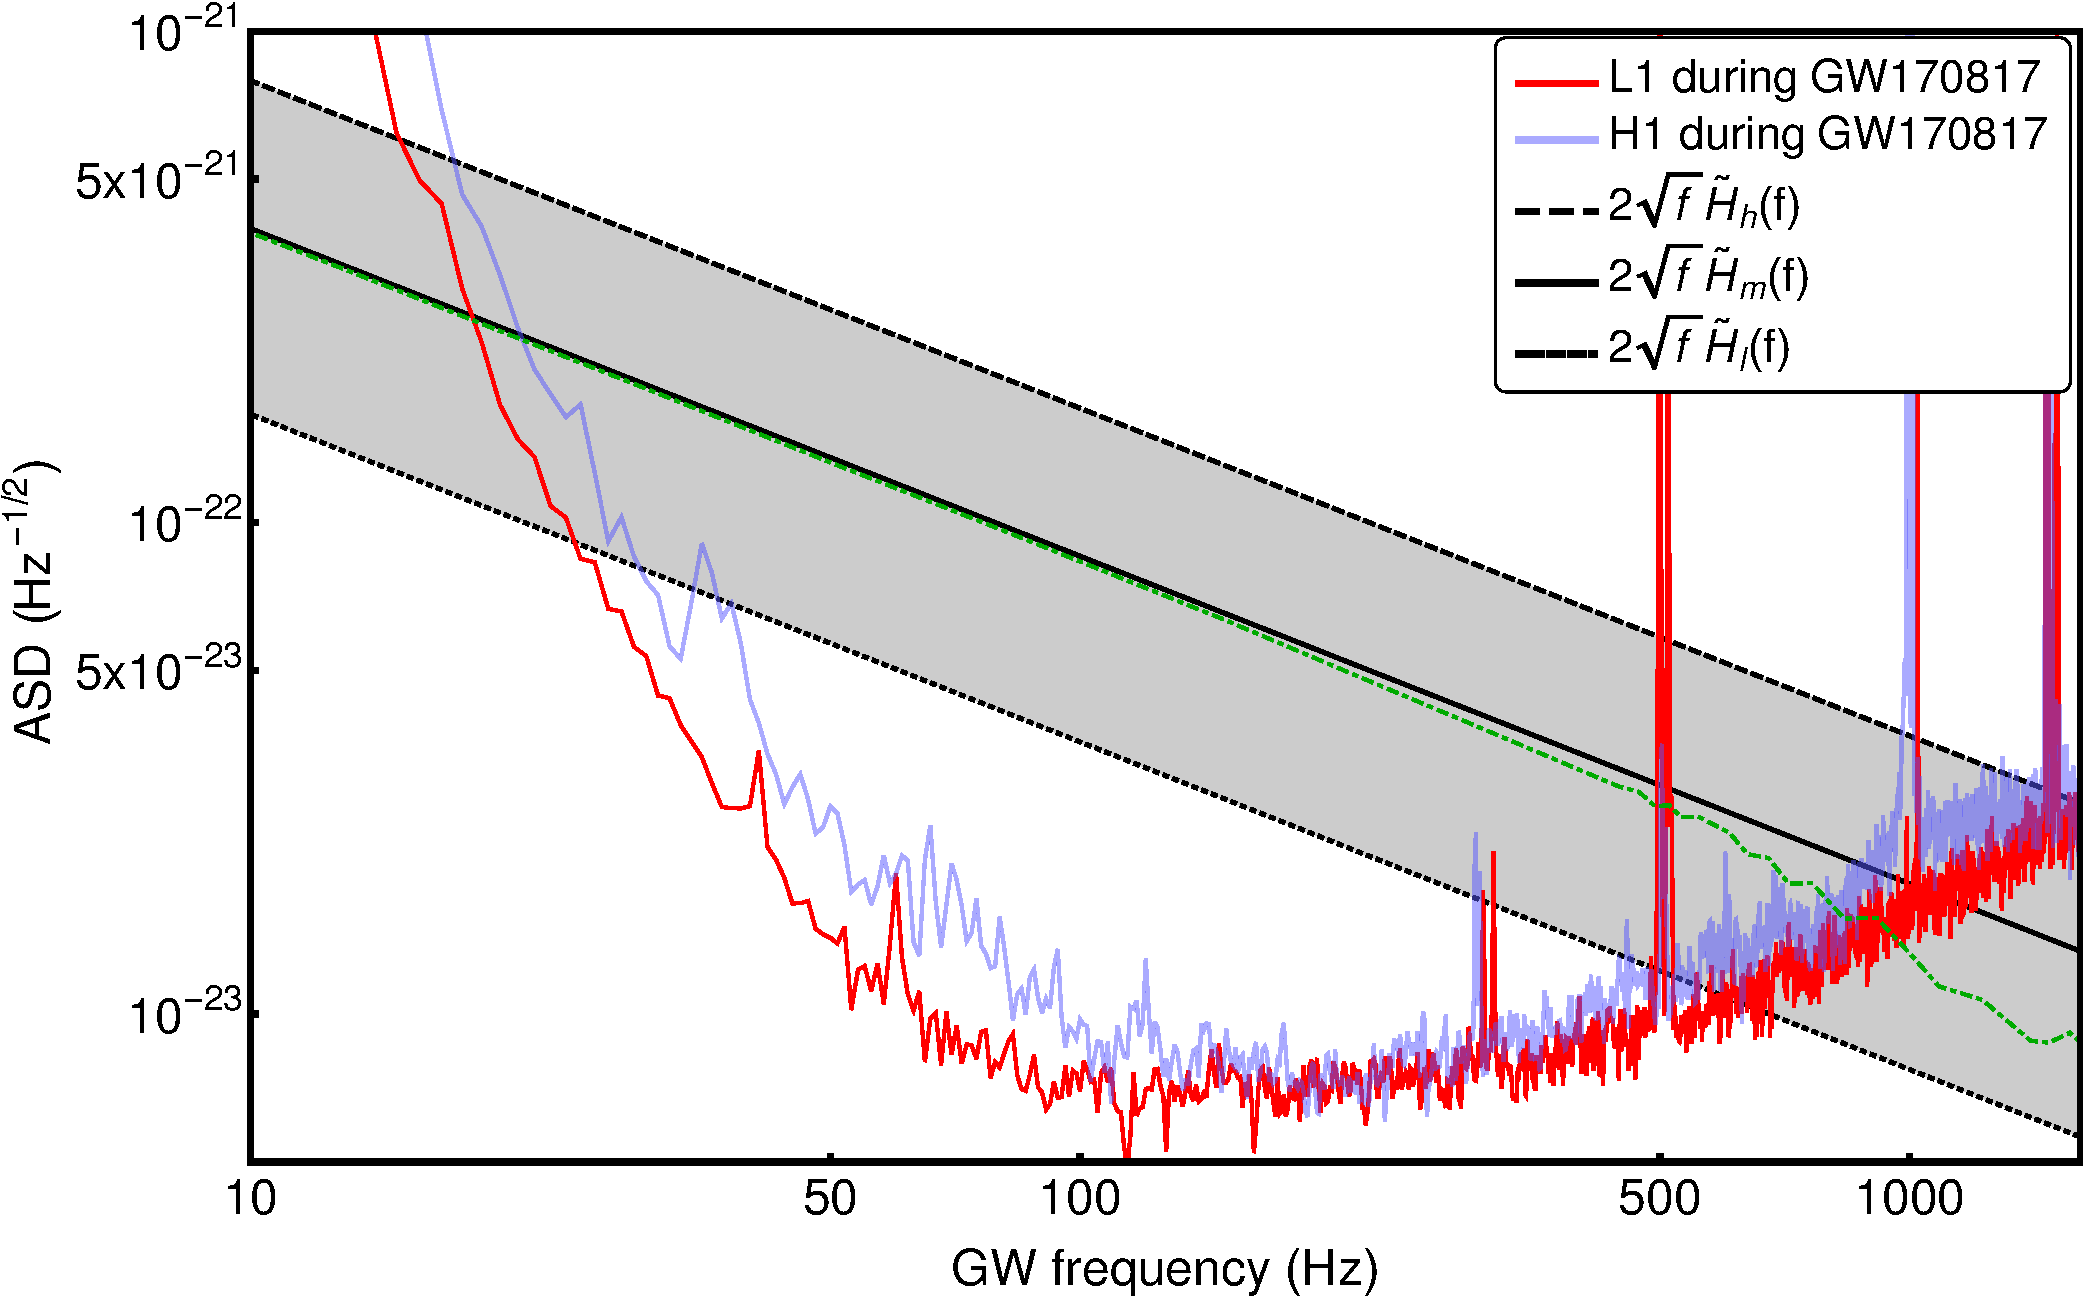
\includegraphics[height=9cm]{../Figures/GW170817_strains.pdf}
\caption{GW170817 as it sweeps from 10\,Hz to $f_\text{ISCO} \simeq1605\,$Hz across our network with ASD (sensitivity) of 
LIGO Livingstone (L1) during the event (the darker red curve).
We also show the Hanford detector's sensitivity in light blue for comparison. The dashed, solid and dotted lines represent the 
response of each interferometer's frequency-domain response ($2\sqrt{f} \tilde{H}_i(f)$ with $i=h,m,l$) to the inspiral of
a binary neutron star system with parameters given in Eq.~(\ref{eq:GW170817_params}).
The variation in strain amplitudes is the result of a given interferometer's orientation and the sky position of the source 
as explained in Sec.~\ref{sec:LIGO_topo} and summarized in Table~\ref{table:network_params}.
In other words, the dashed line is how ``loud'' GW170817 would appear in the data stream of a near optimally oriented IFO with L1's sensitivity
%would be if L1was optimally positioned and oriented 
(quality factor $Q=4/5$). Similarly, the solid line represents the strain in %a randomly oriented IFO with randomized source sky location, hence
the RMS-averaged IFO with L1's sensitivity ($Q=2/5$). %, but with RMS-average over all angles 
%determining source orientation and position. 
Finally, the dotted line represents a pessimistic IFO orientation and source location (sub-optimal configuration)
resulting in a reduction of amplitude to $ 16.7\%$ of the $Q=1$ case. 
The shading represents the region of likelihood for where the strain due to an inspiralling BNS would be. In the case of a three-IFO
network, we would expect all three strains to exist somewhere in the shaded region most of the time and two out of three every time.
%The darker region marks $\text{RMS}\pm(\sqrt{2/5}-2/5)$ translating to an amplitude range of $ 16.7\% - 63.2\%$ of the maximum $\tilde{H}_h(f)$.
%For a randomly located, oriented BNS inspiral, we expect its strain to sweep in the lighter region for one IFO and in the darker region for the other two IFOs.
The dot-dashed (green) curve shows a more realistic strain constructed with data from numerical simulations of Ref.~\cite{Read:2009yp}.
The breakdown of the leading-order $\sqrt{f}f^{-7/6}=f^{-2/3}$ behavior around $f\sim100\,$Hz due to tidal effects is clear.
%Note that although we extend the $\sqrt{f}f^{-7/6}=f^{-2/3}$ power law behavior of the strains all the way to ISCO, in actuality, this  starts breaking down .
}
\label{fig:figGW170817}
\end{figure}
%
%


We can now compute the total SNR of GW170817 as inferred by our network
%%
%
\be
\bar\rho_\text{tot}= \sqrt{\bar\rho^2_h+\bar\rho^2_m+\bar\rho^2_l}= 32.6 \, \label{eq:SNR_total_GW170817} .
\ee
%
%%
This also compares well with the actual value of 32.4. Therefore, we conclude that our imaginary network performs realistically enough to make predictions on the performance of IFOs in the 2020s and 2030s.
%
%
%
%
%
\section{Results: Advance warning times for inspiralling neutron stars}\label{sec:results}
 %\subsection{BNS inspirals at Advanced LIGO-Virgo and the Einstein Telescope}\label{Sec:BNS_2020_2030}
 %Recall that we are interested in the advance warning times that the (near)-future ground-based interferometers can provide for the optical astronomers before the prompt GRB at the end of the merger. 
 Our aim is to foretell GRBs using our network made up of three IFOs with A-LIGO design sensitivity in the 2020s and the Einstein Telescope sensitivity in the 2030s.
 Our predictive capabilities depend on how much advance warning the future networks will give us prior to the prompt merger/GRB.
 Our definition of advance warning is the inspiral time to the merger from a certain threshold instant $\bar{t}$ at which point the network ``agrees'' that there is an inspiral 
 event statistically significant enough to issue warnings to electromagnetic telescopes.
 We define this threshold instant to be given at a frequency $\bar{f}$ when the total SNR equals 15. 
 More specifically, in the case of the Advanced-LIGO-Virgo network (ALV), our statement is that there exists a frequency $\bar{f} < f_\text{ISCO}$ such that
 %
 \be
 \bar\rho_\text{tot}= \sqrt{\left[\rho_h(f_0^h,\bar{f})\right]^2+\left[\rho_m(f_0^m,\bar{f})\right]^2+\left[\rho_l(f_0^l,\bar{f})\right]^2}=15, \label{eq:SNR_bar}%2\tilde{A}_m\, h_0\left[ \int_{f_0}^{{\bar{f}}} df'\, \f{f'^{-7/3}}{S_\text{noise}(f')}\right]^{1/2} =15 .
 \ee
 %
 where $f_0^i$ are given by the solution set to
 %there exists some frequency $f_0 < \bar{f}$ such that
 \be
 \sqrt{S_\text{n}(f_0^i)} = 2\sqrt{f_0^i}\, \tilde{H}_i(f_0^i) \label{eq:f0},\qquad i=h,m,l
 \ee
 %
 with $f_0^i < \bar{f}$. In other words, $f_0^i$ are the initial GW frequencies at which a given inspiral enters the $i$th IFO's sensitivity band. 
 Once we know $\bar{f}$, we can compute the remaining time to the merger, $\tau_\text{insp}(\bar{f})$, using Eq.~(\ref{eq:tau_insp})
 and its 3.5PN-enhanced version from Ref.~\cite{Blanchet_LRR}. This is what we call our advance warning time $T_\text{AW}$.
 For simplicity, we set $m_1=m_2=1.4 M_\odot \implies M_c\simeq 1.219 M_\odot$, which we justified in
 Point 3 of Sec.~\ref{sec:idealizations}. 
 With the masses fixed, the only variable determining $h_0$ is the luminosity distance $D$ as can be seen from Eq.~(\ref{eq:h0}).
 We summarize our procedure in the flow diagram below.
 %
 %
  \begin{figure}[ht!]
 \framebox{\Longstack[l]{Pick $D$}}$\longrightarrow$\framebox{\Longstack[l]{Construct\\ $\tilde{H}_i(f)$}} 
 $\longrightarrow$  \framebox{\Longstack[l]{Compute $f_0^i$\\ from Eq.(\ref{eq:f0})}} $\longrightarrow$  \framebox{\Longstack[l]{Compute $\bar{f}$\\ from Eq.(\ref{eq:SNR_bar})}}
 $\longrightarrow$  \framebox{\Longstack[l]{Compute $T_{AW}=\tau_\text{insp}(\bar{f})$\\ from Eq.~(\ref{eq:tau_insp})}}
  \caption{Flow diagram summarizing our procedure for computing advance warning times $T_\text{AW}$ with the Advanced-LIGO-Virgo network. 
  We will compute $T_\text{AW}$ for the case of $M=2.8M_\odot$ BNS system inspiralling at $D=50,100,200\,$Mpc. 
  %for A-LIGO and $D=200,400,1000\,$Mpc for the ET.
  }\label{fig:flow}
\end{figure}

%
 %\noindent
 %$ \boxed{{\scriptstyle \text{Pick $D$}}} \longrightarrow\boxed{\scriptstyle\text{Construct $\tilde{H}_m(f)$}}\longrightarrow\boxed{{\scriptstyle \text{Compute $f_0$ from Eq.(\ref{eq:f0})}}}\longrightarrow\boxed{\scriptstyle\text{Compute $\bar{f}$ from Eq.(\ref{eq:SNR_bar})}}\longrightarrow\boxed{{\scriptstyle \text{Compute }T_{AW}=\tau_\text{insp}(\bar{f})}} $\\
 %
 %
 We consider inspiralling BNS systems at $D=50,100,200\,$Mpc as our canonical sources for the ALV network.  
 %and BNS systems at $D=200, 400, 1000\,$Mpc for the ET network. 
 For each case, we compute $\bar{f}$ from Eq.(\ref{eq:SNR_bar}) with which we then compute $T_\text{AW}=\tau_\text{insp}(\bar{f})$.
  %
%\be
%\bar{\rho}_\text{tot}\equiv{\rho}_\text{tot}(f_0,\bar{f})= \sqrt{\left[{\rho}_h(f_0,\bar{f})\right]^2+\left[{\rho}_m(f_0,%\bar{f})\right]^2+\left[{\rho}_l(f_0,\bar{f})\right]^2} \label{eq:SNR_bar_total} 
%\ee
%
%to further strengthen our detection criterion (\ref{eq:SNR_bar}). 
%Finally, we will present 
We additionally calculate 
the total accumulated SNR from $f_0$ to $f_\text{ISCO}$ for each inspiral using%sweeping the A-LIGO and ET network bandwidths
 %
\be
\bar{\rho}_\text{F}\equiv\sqrt{\left[{\rho}_h(f_0^h,{f}_\text{ISCO})\right]^2+\left[{\rho}_m(f_0^m,{f}_\text{ISCO})\right]^2+\left[{\rho}_l(f_0^l,{f}_\text{ISCO})\right]^2} \label{eq:SNR_bar_FINAL} .
\ee
%
%
We will introduce the expressions for ET's $\bar\rho_\text{tot},\bar\rho_F$ in Sec.~\ref{Sec:ETB}.
To compute the SNRs defined above for the ALV network we require IFO noise data for which
we use the ASD for the BNS-optimized A-LIGO design sensitivity expected to be attained ca. 2020 \cite{LIGO2020}. 
This is plotted as the thick red solid curve in Fig.~\ref{fig:LIGO2020}.
Sweeping across the detector's frequency bands are RMS-averaged GW strains ($\tilde{H}_m$) due to BNS inspirals at various luminosity distances.
Each RMS-averaged strain is accompanied by its shaded region ranging from an optimally oriented strain ($\tilde{H}_h$) to a sub-optimally oriented strain ($\tilde{H}_l$). These regions were first explained in Sec.~\ref{sec:GW170817} and shown in Fig.~\ref{fig:figGW170817}.
Recall that this is our way of representing the response of a three-IFO network to a single source, i.e., we map three different IFO responses due to a single source to a single IFO's response to three different sources differing in amplitudes as listed in Table~\ref{table:network_params}.
The height of a given strain above the detector sensitivity provides a good \emph{visual} estimation for the corresponding SNR,
but the reader should keep in mind that the actual computation involves a ratio, not a difference, as shown, e.g., in Eq.~(\ref{eq:SNR}).
%
%
%
\subsubsection{Forecasting GRBs in the 2020s with the Advanced LIGO-Virgo Network}\label{Sec:ALIGO2020}
We now compute the advance warning times that A-LIGO can provide us in the case of BNS inspirals at $D=50, 100,200\,$Mpc.
Fig.~\ref{fig:LIGO2020} displays the strains due to these inspirals in the same fashion as
Fig.~\ref{fig:figGW170817}: the solid (black), dotted (blue), and dashed (green) lines represent the RMS-averaged characteristic strains, $2\sqrt{f}\tilde{H}_m(f)$, at luminosity distances of $D=50, 100, 200\,$Mpc, respectively, with the shaded regions covering the range
between the optimally oriented case and the sub-optimal case.
%
%
\begin{figure}[ht!]
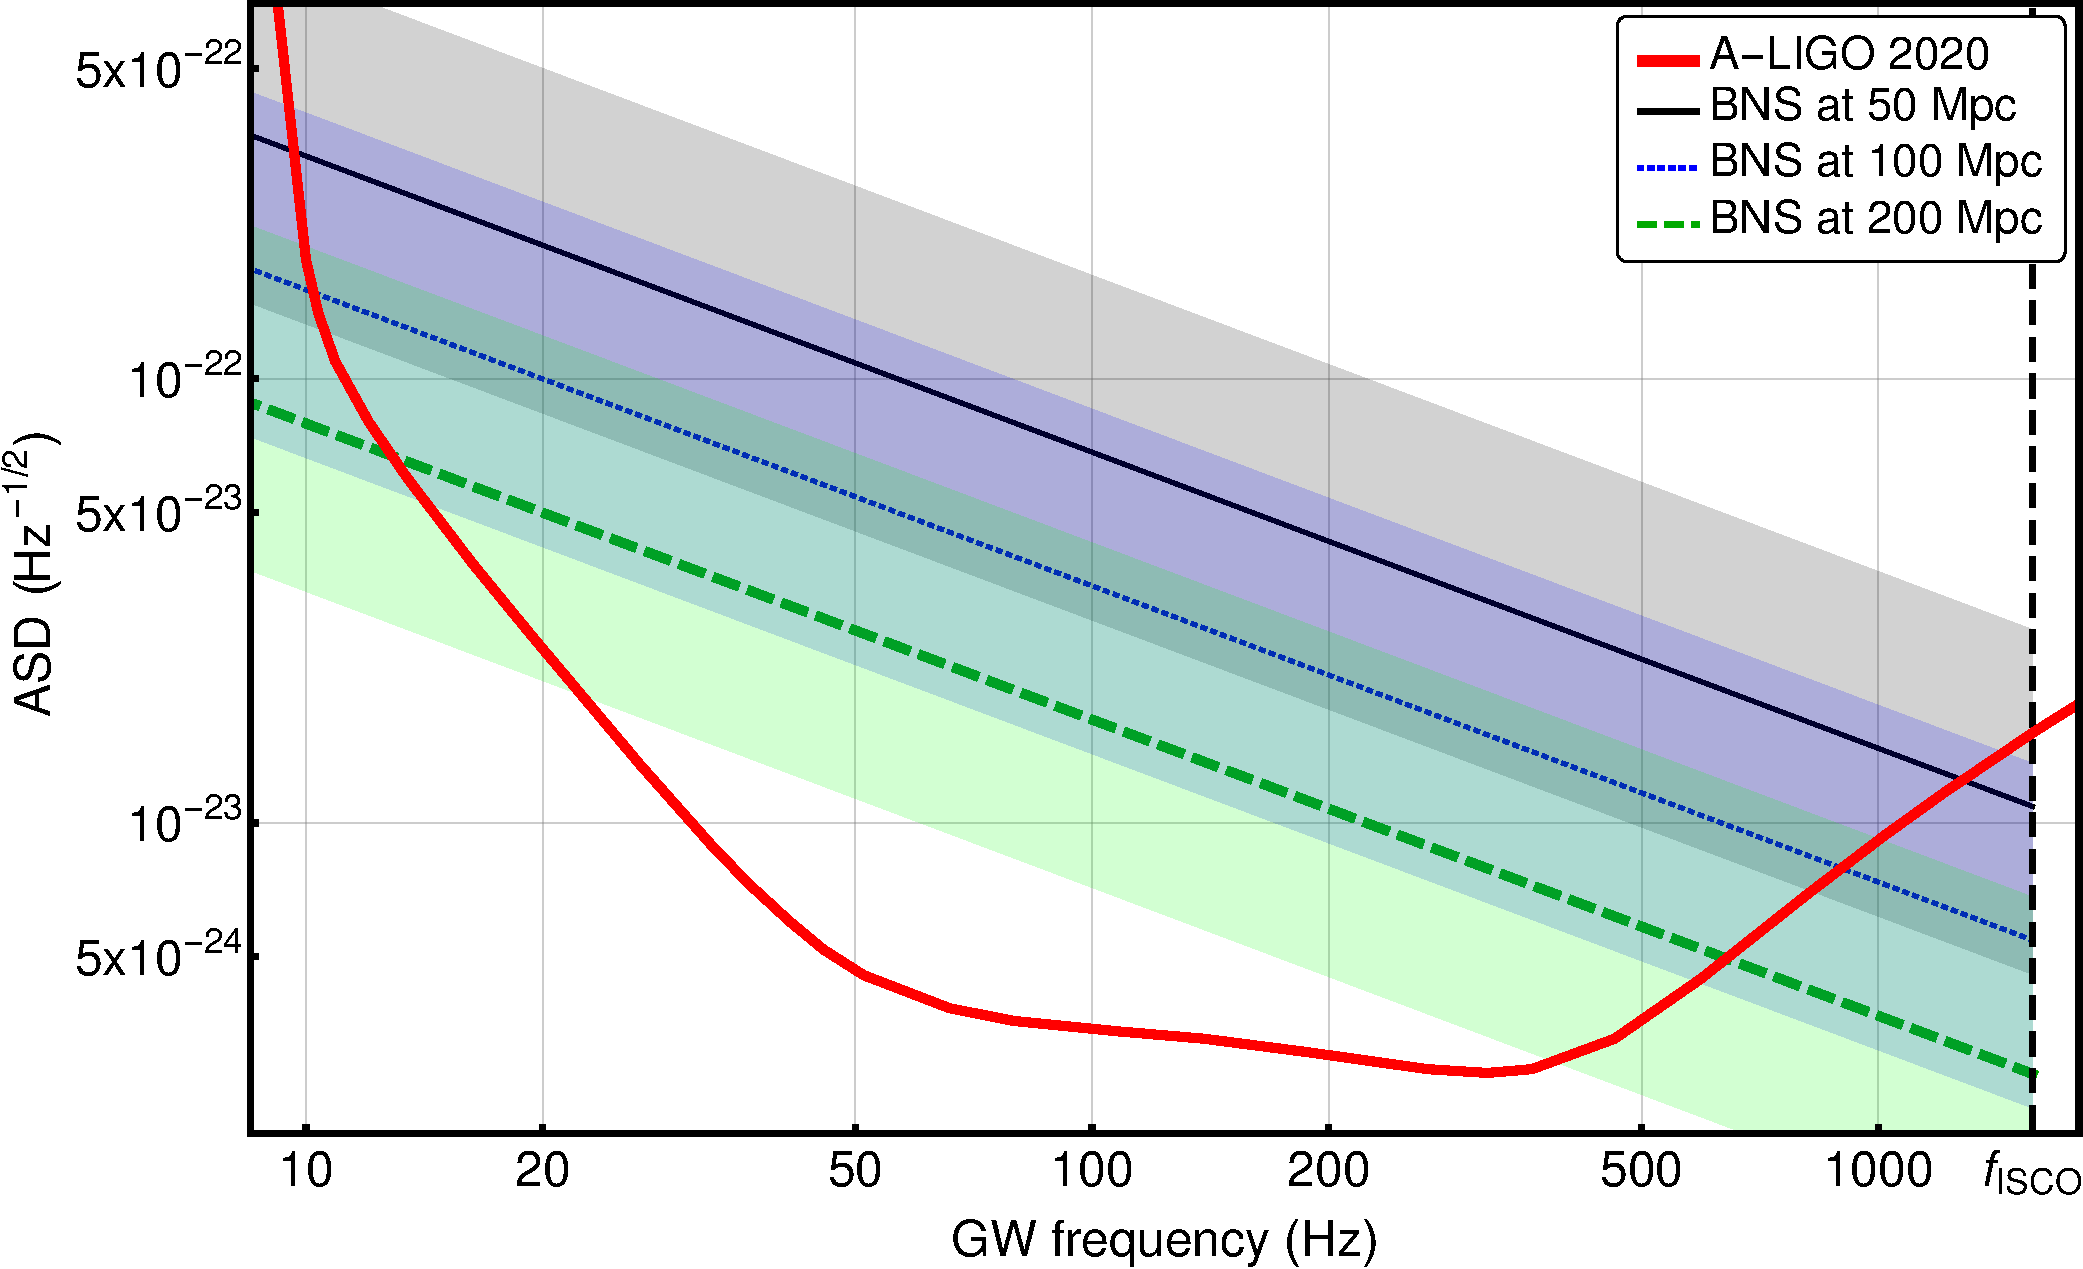
\includegraphics[width=\linewidth]{../Figures/ALigo_strains.pdf}
\caption{Typical $M=2.8 M_\odot$ BNS inspirals sweeping across the Advanced LIGO-Virgo network in the 2020s.
These may be the harbingers of short GRBs.
%inspiralling BNS systems sweeping across the most sensitive interferometer frequencies.
The solid (black), dotted (blue), and dashed (green) lines are the RMS-averaged strains ($2\sqrt{f}\tilde{H}_m(f)$) at luminosity distances of $D=50, 100, 200\,$Mpc, respectively. The accompanying shaded regions cover the region of likelihood for a three-IFO network as explained in Fig.~\ref{fig:figGW170817}.
The vertical dashed (black) line marks the ISCO frequency $f_\text{ISCO} \simeq 1571\,$Hz at which point we terminate the inspirals,
but as can be seen, the SNR hardly increases beyond $\sim 1000\,$Hz.
%Recall that we deliberately neglect the tidal and strong-field effects that modify the plotted $f^{-2/3}$ power law beyond $\sim 100\,$Hz.
%we artificially extend the leading-order $f^{-2/3}$ power law past $f\sim 100\,$Hz at which point tidal effects actually visibly modify this behavior.}
}
\label{fig:LIGO2020}
\end{figure}
%
%

The computation follows the procedure outlined in Fig.~\ref{fig:flow}. We use numerical root finding to determine $\bar{f}$ and $f_0^i$ for all three values of $D$. 
The computation of SNRs and advance warning times is straightforward. 
We summarize our results in Table \ref{table:LIGO2020} where we present both the 0PN and the 3.5PN results for the advance warning times
$T_\text{AW}$. As can be seen from the values for $T_\text{AW}$ in the table, we can at best expect 85\,seconds of early warning time.
This time increases to 2\,minutes in the case of another GW170817-like event with $D=40\,$Mpc.
The current best estimate for the event rate of BNS inspirals is $ 1540^{+3200}_{-1220}\,$Gpc$^{-3}$yr$^{-1}$, inferred from the O1 and O2 observing periods of Advanced LIGO \cite{GW170817}.
This translates to $\approx 0.1$ event per (40-Mpc)$^3$ per year with the upper limit $\approx 0.3$. So we can at best hope to detect
one 40-Mpc inspiral per a three-year period.
Therefore, we do not expect to be able forecast GRBs in the Advance LIGO-Virgo era given that we might at best have a couple of minutes of warning time. 
%we prefer to remain optimistic about the prospects of forecasting at least one GRB in the 2020s. %that this latency can be reduced to minutes.
%if we dare to entertain peak CPU computation rates of $\sim 10^{13}\,$flops/sec for 2020 then $\sim 100$ computing cores would suffice to match-filter $10^5$ templates {\bf in how much time?} extrapolating on the results of Ref.~\cite{Cannon:2011vi}.
%
%Regardless of the future capabilities of search algorithms, 
%So if the automated warning routines in the 2020s become sophisticated enough to send out alerts in $\sim 1\,$minute then
%there might be hope to electromagnetically observe one to three GRBs or the resulting optical transient using 
%the Large Synoptic Survey Telescope \cite{LSST} might observe the resulting optical transient. 
%In the case of GW170817 it took nearly 11 hours to find this optical transient \cite{GBM:2017lvd}. 
%As is clear from Table~\ref{table:LIGO2020} we can hope to electromagnetically observe only the $D\lesssim 50\,$Mpc GRBs.
%
\begin{table}[h]
\centering
\begin{tabular}{lcccccc}
\hline
$D\,$(Mpc) & $\bar{f}\,$(Hz) &{}& $T^{0PN}_\text{AW}$(sec) &\hspace{1mm} & $T^{3.5PN}_\text{AW}$(sec)& $\bar{\rho}_F$\T\B\\
\hline
50 & 25.3 & & 84.25 & & 85.86 & 70.3 \T\\
100 & 41.6 & & 22.39 & & 22.86 & 35.2 \\
200 & 121.3 & & 1.291 &\quad & 1.300 & 17.6 \\
\hline
\end{tabular}
\caption{The Advanced LIGO-Virgo (ALV) network's potential for providing advance warning times, $T_\text{AW}$, 
to electromagnetic observatories for inspiralling binary neutron stars at luminosity distances of $D=50,100,200\,$Mpc. 
$\bar{f}$ is the frequency at which the  signal-to-noise ratio (SNR) accumulated by the ALV network reaches 15. 
$\bar{\rho}_F$ is the total accumulated network SNR for each inspiral. We present both the Newtonian (0PN) 
and the 3.5 post-Newtonian result for the advance warning times.}\label{table:LIGO2020}
\end{table}
%
%
Be that as it may,
%In addition to potentially alerting the E\,\&\,M community, 
the ALV network will accumulate impressive SNRs 
(see $\bar{\rho}_F$ in Table~\ref{table:LIGO2020}) for BNS inspirals out to 100\,Mpc.
%Monte-Carlo simulations of BNS systems indicate that 
As the measurement errors for the system parameters are proportional to $\bar\rho^{-1}_F$ \cite{Cutler:1994ys},
systems that yield high SNRs ($\bar\rho_F\gtrsim 40$) will enable (i) high precision measurements of 
$M_c, M$ \cite{Farr:2015lna}; (ii) sky localization to $\lesssim 5\,\text{Deg}^2$ \cite{Rodriguez:2013oaa};
(iii) $ \lesssim 10\%$ precision in the inferred NS masses \cite{Rodriguez:2013oaa} and the effective spin parameter $\chi_\text{eff}$ \cite{Zhu:2017znf}; and
(iv) restrictions on the equation of state and the tidal deformability
parameters of neutron stars \cite{Read:2009yp, Andersson:2009yt, PhysRevD.89.103012, PhysRevD.91.043002}.
We should caution the reader that such high-SNR systems will make up $\lesssim 1\%$ of the population of BNSs detected by 
the ALV network \cite{Sathyaprakash:2012jk}.

\subsubsection{Forecasting GRBs in the 2030s using the Einstein Telescope}\label{Sec:ETB}
We now wish to quantify the forecasting capabilities of Einstein Telescope. To this end, we consider the inspiral of BNS systems
at luminosity distances of $100,200,400,1000\,$Mpc entering the ET band. 
These correspond to cosmological redshifts of $z\approx 0.0222,0.0437, 0.085, 0.198$, respectively.
To compute these, we used a flat $\Lambda$CDM model ($\Omega_k=0$) with the latest Planck satellite parameters: 
$\Omega_\Lambda = 0.6911, \Omega_m = 0.3089, H_0 = 67.74\,$km\,s$^{-1}\,$Mpc$^{-1}$ \cite{Planck2015}. % with negligible ra yielding and $\Omega_r \lesssim 10^{-4}$.
It is then straightforward to translate $D$ to $z$ (cf. Ref.~\cite{Hogg:1999ad}).


The SNR accumulated in ET from each inspiral is obtained by a modification to Eq.~(\ref{eq:ET_SNR})

%
\be
\bar\rho_{\text{ET}}(f_0,f)\equiv \f{36}{25}A^2 h_0^2\, (1+z)^{-1/3}\int_{f_0}^{f} d f'\, \f{f'^{-7/3}}{S^\text{ET}_n(f')} \label{eq:ET_SNRv2},
\ee
where $f_0$ is the GW frequency at which the emitted GWs enter ET's detection band, i.e, $f_0 < f_\text{ISCO}$ such that
%
 \be
 \sqrt{S^\text{ET}_\text{n}(f_0)} = 2\sqrt{f_0}\, \tilde{H}_\text{ET}(f_0, D) \label{eq:f0_ET}\,
 \ee
 %
with $\tilde{H}_\text{ET}(f, D)$ given by the redshifted version of Eq.~(\ref{eq:H_delta})
%
\be
\tilde{H}_\text{ET}(f, D) = \f{1}{2}\sqrt{\f{3}{10}}\, \f{c}{D}\f{1}{(1+z)}\left(\f{G \mathcal{M}_c}{c^3}\right)^{5/6} f^{-7/6}\, , \label{eq:H_delta_redshifted}
\ee
%
where recall $\mathcal{M}_c = (1+z)M_c$.
For the detector noise $\sqrt{S^\text{ET}_n(f)}$, we adopt the ASD for the B and C configurations known as ET-B and ET-C, respectively \cite{Hild:2010id} which we plot as the solid dark (red) and light (brown) curves in Fig.~\ref{fig:ETB2030}.
Sweeping across these are four BNS inspirals at $D=100,200,400,1000\,$Mpc represented by solid (black), dotted (blue), dashed (green),
and dot-dashed lines (gray), respectively. These strains sit much higher than the detector noise
compared with those in Fig.~\ref{fig:LIGO2020} which foretells us that the SNRs accumulated in the ET band will be much higher, 
thus yielding much longer advance warning times as we show in Table~\ref{table:ET}.
%As shown, Einstein Telescope is sensitive enough to accumulate more SNR in this $f>f_\text{ISCO}$ regime.

\begin{figure}[ht!]
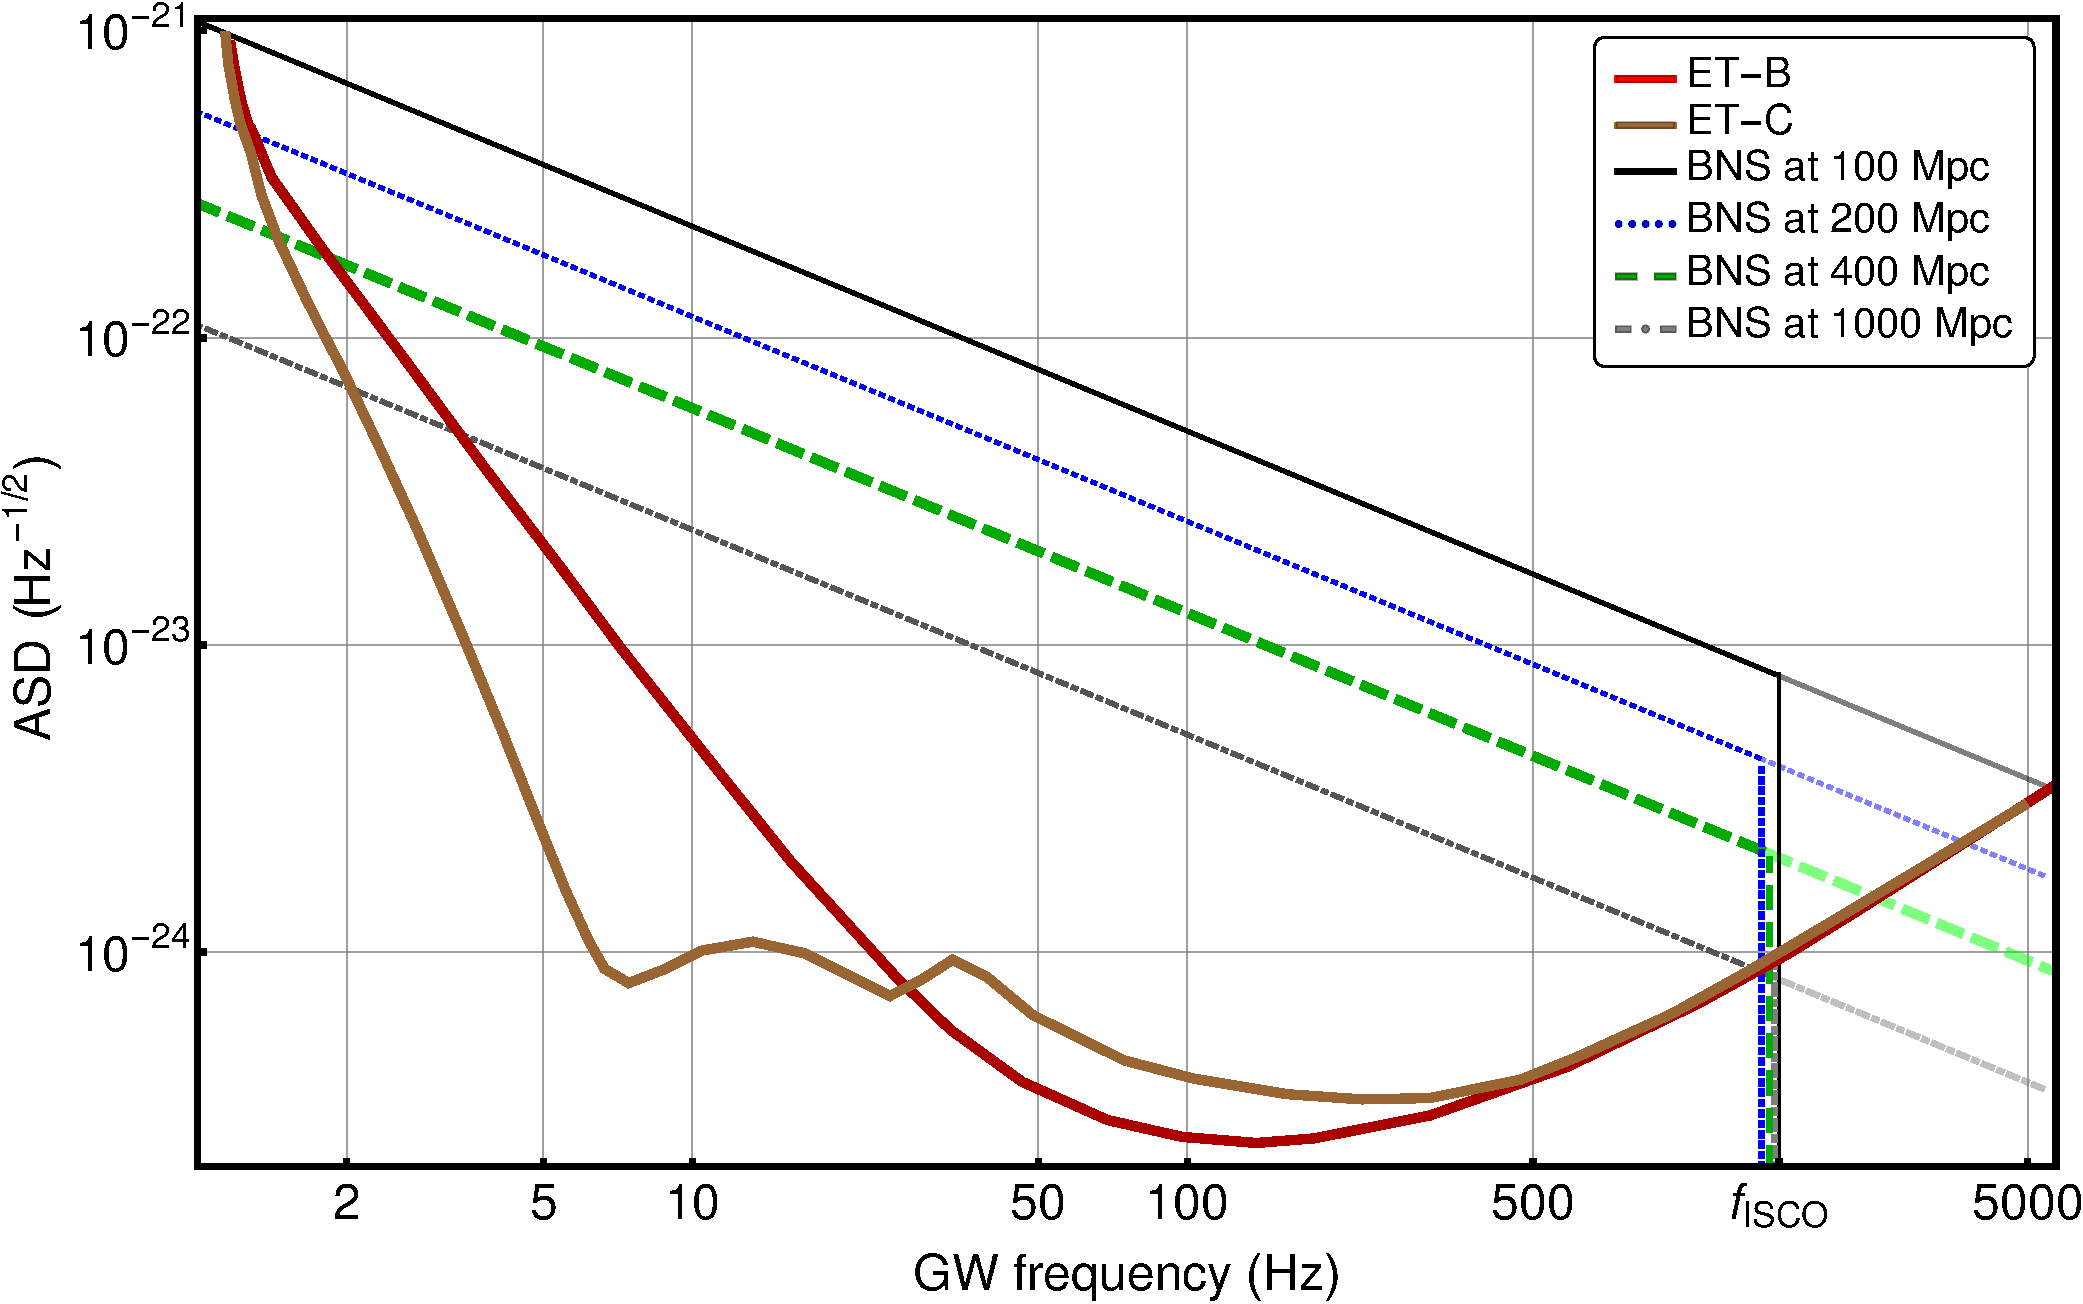
\includegraphics[width=\linewidth]{../Figures/ET_strains_redshifted.pdf}
\caption{Typical GW sources that may be harbingers of GRBs in the 2030s: $1.4 M_\odot-1.4 M_\odot$ inspiralling BNS systems sweeping across 
the Einstein Telescope's sensitivity band for both B and C configurations.
The solid (black), dotted (blue), dashed (green), and dot-dashed lines (gray) lines are the redshift-corrected
RMS-averaged strains, $2\sqrt{f}\tilde{H}_\text{ET}(f,D)$, at luminosity distances of $D=100, 200, 400, 1000\,$Mpc, respectively. 
The vertical lines with correspondingly identical patterns (colors) mark the redshifted ISCO frequencies ($(1+z)^{-1} f_\text{ISCO}$) at which point we terminate each inspiral.
As the true ISCO frequency is likely larger than $f_\text{ISCO}$ \cite{Marronetti:2003hx}, the inspirals would continue to nearly 2\,kHz indicated by the 
faded lines in the plot (drawn to 5\,kHz for aesthetic reasons).
%However, numerical simulations indicate that the actual ISCO is smaller than the Schwarzschild value $6GM/c^2$ hence the true ISCO
%frequency is greater than $f_\text{ISCO}$ used here.
%As shown, Einstein Telescope is sensitive enough to accumulate more SNR in this $f>f_\text{ISCO}$ regime.
%Once again, keep in mind that we artificially extended the leading-order $f^{-2/3}$ power law past $f\sim 100\,$Hz at which point tidal effects actually visibly modify this behavior.
}
\label{fig:ETB2030}
\end{figure}
%
%
To determine $T_\text{AW}$ we once again impose the threshold SNR of 15 which, the reader may recall, 
is our detection criterion for sending out warnings to electromagnetic observatories. Thus, rewriting Eq.~(\ref{eq:SNR_bar}) in the case of ET, we define $\bar{f}_\text{ET}$ as the solution to
%
\be
\bar\rho_\text{ET}(f_0,\bar{f}_\text{ET}) = 15 \label{eq:ET_fbar},
\ee
%
where $f_\text{ISCO}$ is now the redshifted version of Eq.~(\ref{eq:f_isco}), equalling $1537, 1505, 1448, 1311\,$Hz, respectively.
$\bar{f}_\text{ET}$ then gives us our redshift-accounted advance warning time via $T_\text{AW}=\tau_\text{insp}(\bar{f}_\text{ET})$ using Eq.~(\ref{eq:tau_insp_redshifted}) which we can slightly improve by using the 3.5PN expression. 
Therefore, we proceed as summarized in Fig.~\ref{fig:flow} and compute the 0PN and 3.5PN advance warning times 
for all four inspirals in both the ET-B and ET-C bands.
The latter computation involves rescaling the PN parameters $x$ and $\Theta$ to $(1+z)^{2/3} x$ and $(1+z)^{-1}\Theta $ (see Sec.~9.3 of 
Blanchet's review \cite{Blanchet_LRR} for details).
The final accumulated SNR is given by
%
\be
\bar\rho_{F}\equiv \bar\rho_\text{ET}(f_0,f_\text{ISCO})  .\label{eq:rhoF_ET}
\ee
%
Table~\ref{table:ET} summarizes our results for both ET-B and ET-C where we chose to only display the 3.5PN-accurate inspiral time as $T_\text{AW}$,
but we computed this quantity via both 0PN and 2PN expressions as a check.


\begin{table}[h]
\centering
\begin{tabular}{l|ccccccc}
%toprule
\hline
$D\,$(Mpc) & \multicolumn{3}{c}{ET-B} &  & \multicolumn{3}{c}{ET-C}\T\B\\
\hline
{}& $\bar{f}\,$(Hz) & \ \hspace{7mm} $T_\text{AW}$ \ \hspace{7mm} & $\bar{\rho}_{F}$ &{} & $\bar{f}\,$(Hz) & \ \hspace{5mm} $T_\text{AW}\hspace{12mm}$& $\bar{\rho}_{F}$\T\B\\
%midrule
100 & $\approx\,$6.72 &  47.0\,minutes & 306.0 &{\qquad} & $\approx\,$3.27 & 5.34\,hours\ & 365.4\T\\
200 & $\approx\,$11.2 & 11.6\,minutes & 152.4 &{\qquad} & $\approx\,$4.10 & 2.87\,hours\ & 182.1 \\
400 & $\approx\,$18.2 & 3.00\,minutes & 75.74 &{\qquad} & $\approx\,$5.06 & 1.51\,hours\ & 90.48\\
1000 & $\approx\,$41.3 &17.2\,seconds & 29.79& \qquad &    $\approx\,$6.76 & 35.6\,minutes & 35.60  \\
% OLD version
%100 & 6.7237 &  2818 & 306.0 &{\qquad} & 3.2692 & 19212 & 365.4\T\\
%200 & 11.2104 & 698.6 & 152.4 &{\qquad} & 4.1028 & 10138 & 182.1 \\
%400 & 18.2234 & 179.8 & 75.74 &{\qquad} & 5.0607 & 5437 & 90.48\\
%1000 & 41.3537 &17.2 & 29.79& \qquad & 6.7553 & 2138 & 35.60  \\
\hline
%bottomrule
\end{tabular}
\caption{Forecasting capabilities of Einstein Telescope summarized. We can expect over \emph{five} hours of early warning for nearby sources. 
ET-B and ET-C refer the different configurations shown in Fig.~\ref{fig:ETB2030}. For the advance warning times, we only present the result of the more accurate 3.5PN computation. $\bar{f}$ is the threshold frequency at which
ET-B/C accumulate SNR of 15 which we take to be our detection criterion. Note that both $T_\text{AW}$ and $\bar\rho_F$ are larger for ET-C
due to its improved sensitivity in the $f\lesssim 30\,$Hz regime compared to ET-B as it is clear in Fig.~\ref{fig:ETB2030}.
These results and those of Table.~\ref{table:LIGO2020} are summarized in Fig.~\ref{fig:summary}.}\label{table:ET}
\end{table}
%
%
As the results of Table~\ref{table:ET} indicate, ET-B will provide $\sim 10 - 50\,$ minutes of warning time for BNS inspirals at $D\lesssim 200\,$Mpc.
Instead of speculating whether or not this is enough to forecast GRBs, we turn our attention to ET-C's forecasting capabilities.
As can be seen from Fig.~\ref{fig:ETB2030}, ET-C's increased sensitivity in the $f\lesssim 30\,$Hz regime will significantly lengthen the advance warning times.
This is best highlighted by the sixth colum of Table~\ref{table:ET}, 
where we show that ET-C will provide up to five hours of early warning time for nearby ($D\lesssim 100\,$Mpc) neutron star mergers.
Moreover, BNS inspirals as far as 200\,Mpc (the ALV network's horizon distance) will persist in the ET-C sensitivity band for a few hours after their initial detection.
Current BNS merger rate, inferred from A-LIGO's O1-O2 periods, implies that $\sim 40$ to $\sim600$ sources within a volume of $(200\,\text{Mpc})^3$ will be detected yearly by ET.
Given Moore's law and new search approaches based on deep learning (\cite{Gabbard:2017lja}) we speculate
that the advances in the detection, localization and early-warning algorithms in the next decade will reduce the required early
warning time to less than an hour; thus we set $T_\text{AW} = 1\,\text{hour}$ and obtain corresponding BNS horizon distances of $D_H=87,613\,$Mpc ($z\approx 0.02,0.127$) for ET-B and ET-C, respectively.
In other words, all inspiralling BNSs closer than $D_H$ will give us more than an hour's leeway before the GRB (assuming detection SNR of 15 as always).
The volume set by $D=D_H$ translates to a BNS merger rate of $\mathcal{O}(1)$ for ET-B and
$\approx 355^{+730}_{-280}\,\text{year}^{-1}$ for ET-C. Additionally, each source within $D_H$ will accumulate $\bar\rho_F \gtrsim 420, 58$ over its inspiral
in the ET-B, ET-C bands, respectively. These are summarized in Table~\ref{table:horizon}.

Both Tables~\ref{table:ET} and \ref{table:horizon} clearly show that ET will yield superb SNRs for sources out to 1\,Gpc. Given that
it takes $\gtrsim \mathcal{O}(1)\,$\emph{day} for a BNS source to inspiral from $f_0\sim 1\,$Hz to $\bar{f}$ of Eq.~(\ref{eq:ET_fbar}),
we can expect ET to localize sources within the horizon distance to $\lesssim 1\,\text{deg}^2$ \cite{Mills:2017urp}.
As the ET construction/commissioning timeline is currently uncertain, we can only speculate that ET-C will be operational after 2030 
(this is roughly in line with the milli-Hertz space interferometer LISA's timeline \cite{Audley:2017drz}).
It is also reasonable to speculate that by that time the detection, localization and early-warning algorithms will have become sufficiently sophisticated
to alert the electromagnetic observatories within an hour of the initial detection (SNR = 15). 
Therefore, we optimistically conclude that 2030s hold in store real-time observations of dozens of gamma ray bursts.
We summarize our major findings for both the ALV network and ET-B/C in Fig.~\ref{fig:summary}.
%
%
%
\begin{table}[h]
\centering
\begin{tabular}{l|ccc}
%toprule
\hline
 & ET-B & & ET-C\T\B\\
\hline
  $D_H $& 87\,Mpc& &{613\,Mpc}\T\\
  $R(D_H) $& $1^{+2}_{-1}\,\text{yr}^{-1}$&\hspace{5mm} &{$355^{+730}_{-280}\,\text{yr}^{-1}$}\T\\
  $\bar\rho_F(D_H)$ & 420 &&{58}\T\B\\
\hline
\end{tabular}
\caption{Horizon distances of ET-B and ET-C assuming $T_\text{AW} =1\,$hour. $R(D_H)$ is the BNS merger rate within a volume of $D_H^3$
obtained by rescaling the rate inferred from GW170817 \cite{GW170817}. $\bar\rho_F(D_H)$ is the total SNR accumulated in ET by a BNS inspiralling at $D_H$ [see Eq.~(\ref{eq:rhoF_ET})].}\label{table:horizon}
\end{table}
%
%
%
\begin{figure}[ht!]
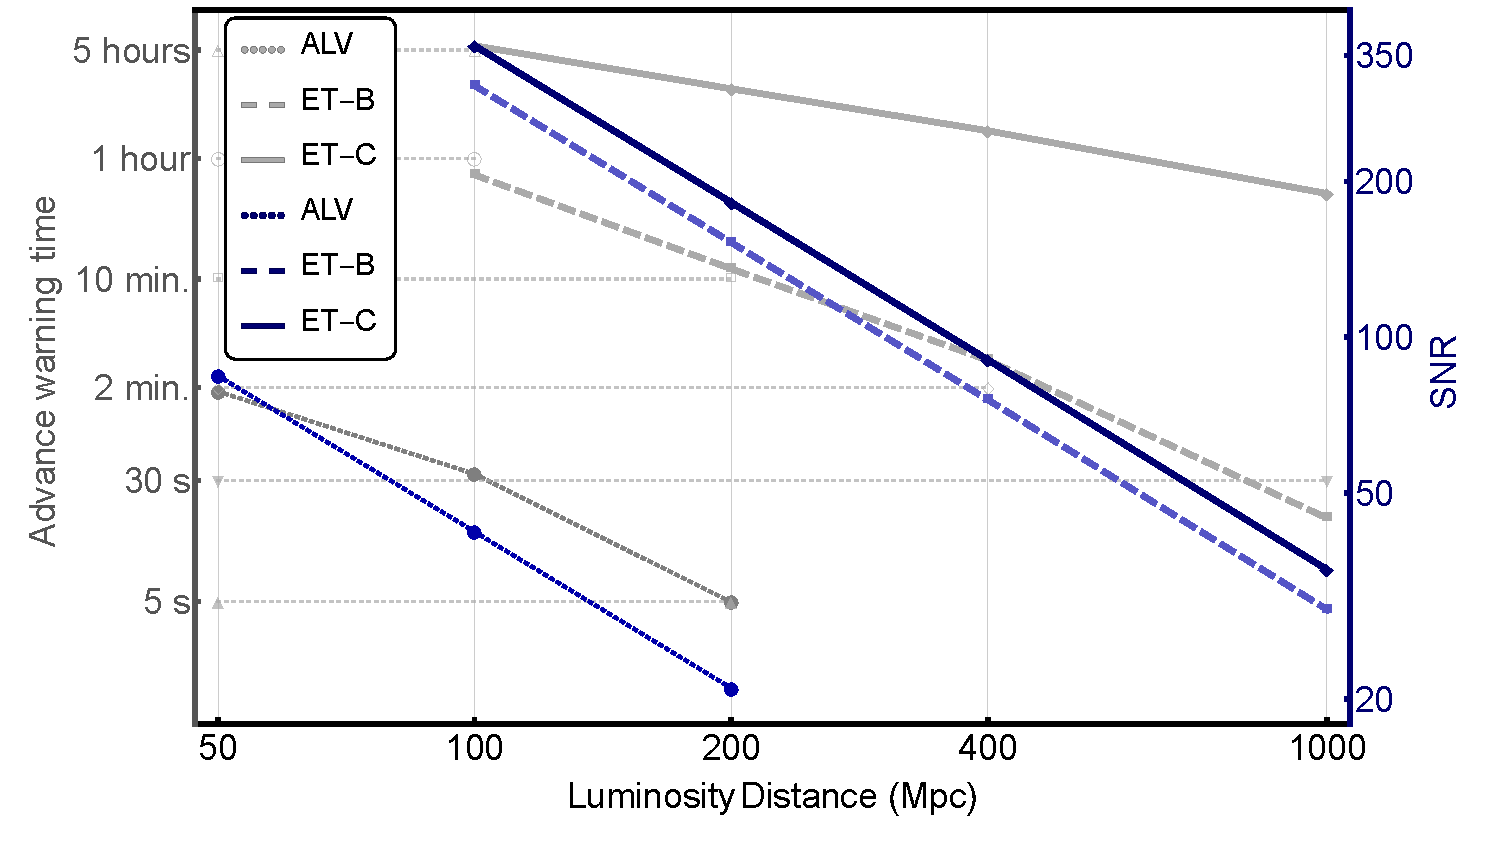
\includegraphics[width=\linewidth]{../Figures/Main_results.pdf}
\caption{Summary of our major findings for both the Advanced-LIGO-Virgo (ALV) network circa 2020 and the Einstein Telescope's B and C configurations
ca. 2030. The light coloured (gray) data shows $T_\text{AW}$ for the ALV network (dotted), ET-B (dashed), and ET-C (solid), respectively.
The connecting light (gray) lines are drawn only for visualization purposes unlike the dark (brown) lines coming from the $D^{-2}$ powerlaw in the SNR [see Eq.~(\ref{eq:ET_SNRsq}] which is plotted on the right axis. 
We used $D=50,100,200\,$Mpc to obtain the ALV results (Sec.~\ref{Sec:ALIGO2020}) and $D\ge 100\,$Mpc for the ET results.}\label{fig:summary}
\end{figure}



% LISA does not see these sources, not sensitive enough!


\section{Binary black hole neutron star systems}\label{sec:BH_NS}
In this section, we investigate the possibility of witnessing the tidal distruption of a neutron star by a black hole before the merger.
The treatment of the inspiral is the same as before, however the fate of the neutron star depends strongly on the system's intrinsic parameters
such as the black hole mass and spin, and the neutron star's equation of state (EOS) and compactness $c_\text{NS}\equiv G M_\text{NS}/(R_\text{NS}c^2)$. 
The evolution of black hole-neutron star (BH-NS) binaries is a very active field of research at the interface of numerical relativity and high-energy astrophysics
(see Ref. \cite{Shibata:2011jka} for a comprehensive review) requiring fully general relativistic magnetohydrodynamic treatment including neutrino transport equations.
The complexity of evolving the dynamics of these systems require large computational resources and long runtimes.
%running on large-scale clusters.
As such, the details are beyond the scope of this article, but we can use a mostly Newtonian treatment to serve our purposes. %, however the numerical simulationshave verified 

A necessary, but insufficient, condition for tidal disruption (TD) is that
\be
\f{2 G M_\text{BH} (c_R R_\text{NS})}{r^3} \gtrsim \f{G M_\text{NS}}{(c_R R_\text{NS})^2} \label{eq:TD_cond1},
\ee
where $r$ is the orbital separation, $R_\text{NS}$ is the radius of the NS and $M$ denotes masses. 
$c_R R_\text{NS}$ is the semi-major axis of the elongated oblate spheroid that represents the tidally distorted shaped of the NS to leading order with
$c_R >1 $. %Setting $m_2= M_\text{BH}, m_1 = M_\text{NS}$, and $r_1=r_\text{NS}$, 
We can roughly take the above condition to be
%
\be
\f{M_\text{BH}}{M_\text{NS}} \gtrsim \left(\f{r}{R_\text{NS}}\right)^3 \label{eq:TD_cond2}.
\ee
%
We wish to maximize the chances of observing a TD event, therefore we ingrain the BH-NS binary with certain desirable features
some of which can be deduced from Eqs.~(\ref{eq:TD_cond1}, \ref{eq:TD_cond2}). These are
%
%
\begin{enumerate}[(i)]
 \item Small separation. As the Newtonian tidal force due to the black hole is proportional to $M_\text{BH}/r^3$, $r$ has to be
 minimized to provide maximum tidal force. 
 However, for $r< r_\text{ISCO}$ the NS simply plunges into the BH; therefore the minium separation is given by the ISCO radius.
 \item Low black hole mass. In the geodesic case, $r_\text{ISCO} \propto M_\text{BH}$, so the Newtonian tidal force roughly scales as $M_\text{BH}^{-2}$. 
 Hence, $M_\text{BH}$ must also be minimized. Once again, there is a lower bound to $M_\text{BH}$ set from astrophysical observations and stellar evolution models.
 Current consensus for this lower bound yields $M_\text{BH} \gtrsim 5 M_\odot$ \cite{Farr:2010tu, Raithel:2017nlc, Ozel:2010su, Wiktorowicz:2013dua}.
 \item High black hole spins. $r_\text{ISCO}$ is much smaller in the case of a prograde NS orbit around a spinning Kerr black hole.
 For instance, for the maximum dimensionless spin value of $a\equiv c J_\text{BH}/(G M^2_\text{BH})=1$, $r_\text{ISCO}$ for prograde orbits is 1/6th of the Schwarzschild value ($6GM_\text{BH}/c^2$) whereas for $a=1$ retrograde orbits, $r_\text{ISCO}$ is 3/2 of the Schwarzschild value.
 With smaller ISCO separation, there is much more tidal force exerted on the NS before it plunges in.
 \item Less compact neutron stars. Eq.~(\ref{eq:TD_cond1}) can be rearranged to isolate $c_\text{NS}$
 on the right hand side. Smaller values for $c_\text{NS}$ mean that TD can occur for $r>r_\text{ISCO}$.
\end{enumerate}
%
We are thus led to set $M_\text{BH} =5 M_\odot$. There is additional motivation to choose low BH mass as 
 $\tau_\text{insp} \propto M_c^{-5/3} = (1+Q)^{1/3}/Q\to Q^{-2/3}$ as $Q\to\infty$ for $Q\equiv m_2/m_1 > 1$, i.e., heavier binaries inspiral faster.
 As we set $M_\text{NS}=1.4 M_\odot$, $c_\text{NS}$ is determined by the radius of the NS constrained in the $9.9 - 11.2\,$km range \cite{Ozel:2016oaf}
 which translates to $0.13\lesssim c_\text{NS} \lesssim 0.15$. We also have $Q  \simeq 3.571$.
%As we wish to avoid discussing the details of the strong-field evolution of the binary, we borrow certain results from the literature to
%justify our choice for the chosen parameters above. 
If we pick the more pessimistic $c_\text{NS} = 0.15$ bound then we must have $Q\lesssim 5$ and $a\gtrsim 0.5$ (prograde) for TD to occur \cite{Ferrari:2008nr}.
and $Q< 3$ in the case of $a=0$ \cite{Kyutoku:2011vz}.
Although the results from each numerical study may somewhat vary what is clear is that we must have high spin and low black hole mass.
This raises an interesting astrophysical question as to whether it is possible to have such light-weight high-spin black holes assuming that
they are spun up by accretion from their secondary (that will later on become a NS) in binary systems, it will have to gain mass.
It is possible that the mass gain pushes $Q$ too high to either cause a direct plunge of the NS before TD or decrease $\tau_\text{insp}$ considerably
to eliminate any chances of getting an advance warning.
However, if the spin of the BH comes from the supernova explosion mechanism itself (as argued for G1915 in Ref.~\cite{McClintock:2006xd} then this is not a problem. 

So we will simply assume that such lightweight, high-spin BHs exist in BH-NS binaries and compute strains and SNRs accordingly.
A quick calculation shows that these systems yield $T_\text{AW} \lesssim 30\,$seconds in the ALV network of 2020s. %in Table \ref{table:LIGO2020}is now less than $ 40\,$ seconds. 
Therefore, we simply focus on the capabilities of ET which we summarize in Table~\ref{table:ET_BH_NS} below.
%
%
%
\begin{table}[h]
\centering
\begin{tabular}{l|ccccc}
%toprule
\hline
$D\,$(Mpc) & \multicolumn{2}{c}{ET-B} &  & \multicolumn{2}{c}{ET-C}\T\B\\
\hline
{}&  \ \hspace{6mm}$T_\text{AW}$ \hspace{8mm} & $\bar{\rho}_{F}$ &{}  & $\hspace{6mm}T_\text{AW} \hspace{10mm}$ & $\bar{\rho}_{F}$\T\B\\
%midrule

100 &   28.2\,minutes & 503 &{\qquad} &  2.15\,hours & 601\T\\
200 & 8.21\,minutes & 251  &{\qquad} & 1.10\,hours & 300 \\
400 &  2.00\,minutes & 124 &{\qquad} & 34.2\,minutes & 148\\
1000 & 14.3\,seconds & 49 &{\qquad} & 13.9\,minutes& 58.5\\
\hline
%bottomrule
\end{tabular}
\caption{Same as Table~\ref{table:ET}, but now for a $5 M_\odot- 1.4 M_\odot$ black hole-neutron star binary.
The SNR is even higher than before, however the advance warning times have decreased significantly.}\label{table:ET_BH_NS}
\end{table}
%
%
\\
\noindent
From the table, we can see that the horizon distance of ET-C for these binaries with $T_\text{AW} \approx 1\,$hour is roughly 200\,Mpc.
Given that the LIGO O1 merger rate for these systems is $ R < 3600\,$Gpc$^{-3}$yr$^{-1}$ \cite{Abbott:2016ymx},
there could be 28.8 such mergers per year within ET-C's horizon distance of $\approx 200\,$Mpc corresponding roughly to $T_\text{AW}\approx1\,$hour.
We must emphasize that this should be viewed
as an upper limit as low-mass, high-spin black holes such as ours above are expected to be rare.
Theoretical studies indicate that $\lesssim 10\%$ stellar-mass BHs have masses $\lesssim 5 M_\odot$ \cite{Fryer:1999ht}.
This seems to be supported at least by observations of galactic black holes \cite{Ozel:2010su}.
Therefore, we realistically expect ET-C to forecast $\lesssim 3$ tidal disruption events per year.
%A better estimation would need to incorporate the percentage of such black holes from population studies and Monte-Carlo simulations,
%however, all of these come with rather large error bars.
%and that no TD occurs for $a=0$. This is roughly consistent with Fig.5 of Ref.~\cite{Hanna:2008um}
%Choosing lower mass implies reduced SNR since $\rho \propto M_c^{5/3} \propto (1+Q)^{1/3}/Q$,
%but even with $m_2=5 M_\odot$, a BH-NS binary is ``louder'' than a BNS system at the same distance. 
%and as we showed in Sec.~\ref{sec:results}, low SNR is not going to be a problem with ET sensitivities out to $D \sim 1\,$Gpc.
%
%It is straightforward to show that this mass bound is only consistent with spinning black holes by substituting the naive Schwarzschild $r_\text{ISCO}$ value 
%into Eq~.(\ref{eq:TD_cond1}) along with $c_R=1.7$ {\bf CITE} which yield $M_\text{BH} \lesssim 4.1 M_\odot$ violating the above BH mass bound.
%ISCO location from NR 
%\be
%\Omega_\text{ISCO} M = 0.068 \left[ 1- \f{0.444}{Q^{1/4}}(1-3.54 C^{1/3})\right] 
%\ee
\section{Outlook}
By constructing representative models of the near-future ground-based gravitational-wave interferometers, we investigated the possibility of
forecasting gamma-ray burts resulting from the merger of two neutron stars.
We showed that we do not expect the Advanced-LIGO-Virgo network to provide such a forecast in the 2020s unless we get extremely lucky
and detect a BNS inspiral in our galaxy which is roughly a one-in-a-trillion shot (in years). %($\sim 1$ per trillion years lucky).
However, the odds completely change in our favour with Einstein Telescope's B and especially C configurations, 
the latter of which is expected to forecast $\gtrsim \ord(10^2)$ GRBs per year as we show in Table~\ref{table:horizon}. 
The same configuration should also forecast up to three tidal disruption events per year in which a high-spin, low-stellar-mass
black hole tidally tears apart its companion neutron star.
The beginning of operation for the C configuration will roughly coincide with the launch of the LISA mission.
Additionally, there are proposals to launch another space interferometer called DECIGO which will operate
between $0.1$ and 10 Hz thus bridging the gap between LISA and the ground-based interferometers \cite{Sato:2009zzb, Kawamura:2006zz}.
With the gravitational-wave sky virtually covered from $10^{-4}$ to $10^3\,$Hz, we will suffer from the 
embarassment of the riches in the 2030s. In short, the future of gravitational and multi-messenger astronomy is bright.

\acknowledgements 
SA thanks Conor O'Toole for endless feedback and Niels Warburton for a careful reading of this article. 
 
 
\bibliographystyle{apsrev4-1}
%\bibliographystyle{plain}
\bibliography{references}

 
 
 
 
 
 
 
\end{document}


Table 6
{}&  \ $T_\text{AW}$(sec) \ & $\bar{\rho}_{F}$ &{}  & \ $T_\text{AW}$(sec)\ & $\bar{\rho}_{F}$\T\B\\
%midrule

100 &   1691 & 503 &{\qquad} &  7834 & 601\T\\
200 & 493 & 251  &{\qquad} & 3975 & 300 \\
400 &  118 & 124 &{\qquad} & 2051 & 148\\
1000 & 14.3 & 49 &{\qquad} & 833& 58.5\\
 